\chapter{Straw-Man Concept design}

This chapter defines the candidate straw-man concepts carried into the system-level trade-off. Each concept is described as a complete mission architecture combining an aerial platform, interaction method, and descent or recovery strategy. The descriptions provide a consistent basis for comparing the concepts in the trade-off. Table~\ref{tab:strawman_concept_overview} gives a compact overview of the candidate concepts selected from the retained design-option-tree branches. The table summarises the main architecture of each concept. 

\begin{table}[H]
    \centering
    \small
    \caption{Candidate straw-man concepts entering the trade-off.}
    \label{tab:strawman_concept_overview}
    \begin{tabularx}{\textwidth}{@{}p{0.04\textwidth} p{0.18\textwidth} X X X@{}}
        \toprule
        \textbf{ID} 
        & \textbf{Concept name} 
        & \textbf{Aerial platform} 
        & \textbf{Interaction principle} 
        & \textbf{Descent/recovery principle} \\
        \midrule

        A &  &  &  &  \\

        B 
        & Cooperative Net-Parafoil Recovery System
        & Carrier eVTOL deploys three net-carrier multirotors and one intervention drone near the target.
        & The net-carrier drones envelop the balloon-payload system using a two-stage cinching net.
        & The secured bundle separates from the drones and descends under a guided parafoil. \\

        C &  &  &  &  \\
        D &  &  &  &  \\
        E &  &  &  &  \\

        \bottomrule
    \end{tabularx}
\end{table}

Table~\ref{tab:common_concept_assumptions} lists the shared assumptions used for concept-level comparison. These assumptions define the target case, operating environment, cueing approach, and recovery conditions applied across the candidate concepts. Any concept-specific assumption is stated in the corresponding concept description.

\begin{table}[H]
    \centering
    \caption{Common assumptions used for all straw-man concepts.}
    \label{tab:common_concept_assumptions}
    \begin{tabularx}{\textwidth}{@{}>{\raggedright\arraybackslash}p{0.30\textwidth} >{\raggedright\arraybackslash}X@{}}
        \toprule
        \textbf{Assumption} & \textbf{Value} \\
        \midrule

        Target balloon size 
        & 2-6 m diameter uncooperative balloon. \\

        Payload-to-balloon tehter length 
        & 2-35 m  \\ 

        Target payload mass 
        & Up to 50 kg suspended payload \\

        Wind condition 
        &  13 m/s sustained wind with 21 m/s gusts \\

        Altitude and range
        & The balloon will be intercepted at up to 6km altitude, at up to 6km ground range \\

        Target cueing source 
        & External cue from radar, observer, airport system, or ground station \\

        Terminal sensing 
        & Onboard tracking will be considered separately from other design choices at this stage due to complexity \\

        Recovery zone 
        & Safe landing/recovery area is flexible and is decided upon during the descent phase of each mission based on weather and the location where the descent starts. \\
        
        \bottomrule
    \end{tabularx}
\end{table}










\section{Baseline Sizing}

All concepts are designed using a common baseline. Below, the method behind the descent profile and an initial estimation of MTOW is illustrated. This is used in all concepts.
\subsection*{Descent Profile}

A critical design driver is the drone's ability to descend while dragging the balloon against sustained winds. At a static equilibrium altitude of 6~km, the balloon volume ($V$) is determined by the buoyancy requirement:

\begin{equation}
    W \cdot g = V \cdot (\rho_{atm} - \rho_{H_2}) \cdot g
\end{equation}

For the given parameters, $V = 87.68\text{ m}^3$, resulting in a radius $r = 2.75\text{ m}$ and a projected area $S = 23.87\text{ m}^2$. 

The drag force ($D$) is calculated using the drag coefficient for a sphere ($C_D = 0.47$) and a design wind speed of 13~m/s (derived from a 21~m/s gust and a 1.62 gust factor). Using the mean air density $\rho$ between sea level and 6~km:

\begin{equation}
    D = \frac{1}{2} \rho v^2 S C_D = \frac{1}{2} \left( \frac{1.225 + 0.66}{2} \right) \cdot 13^2 \cdot 23.87 \cdot 0.47 \approx 894.4\text{ N}
\end{equation}


\subsection*{Power and Mass}
\label{sec:power_mass}

The vehicle mass is estimated using an iterative sizing loop that ensures the Maximum Take-Off Weight ($MTOW$) can support the energy requirements of the mission. The total mass is defined as:
\begin{equation}
    MTOW = m_{batt} + m_{struct} + m_{prop} + m_{fixed} + m_{margin}
\end{equation}
where $m_{struct}$ and $m_{prop}$ are modeled as fractions of the total weight ($f_{struct}$ and $f_{prop}$ respectively). 


The battery mass ($m_{batt}$) is derived from the total mission energy ($E_{total}$), specific energy density ($\rho_{batt}$), and an operational reserve ($R_{res}$):
\begin{equation}
    m_{batt} = \frac{E_{total}}{\rho_{batt} \cdot (1 - R_{res})}
\end{equation}
The total energy is the sum of the power consumed during each flight phase ($i$) multiplied by the phase duration ($t_i$):
\begin{equation}
    E_{total} = \sum P_i t_i = (P_{climb} t_{climb}) + (P_{hover} t_{hover}) + (P_{cruise} t_{cruise}) + (P_{descent} t_{descent})
\end{equation}
The power requirements for each phase are calculated as follows:
\begin{itemize}
    \item \textbf{Hover Power:} $P_{hover} = \frac{1}{\eta_{hover}} \sqrt{\frac{(MTOW \cdot g)^3}{2 \rho A}}$
    \item \textbf{Cruise Power:} $P_{cruise} = \frac{(\frac{1}{2} \rho V^2 S C_D) \cdot V}{\eta_{prop}}$
    \item \textbf{Climb Power:} $P_{climb} = \frac{MTOW \cdot g \cdot v_{climb}}{\eta_{climb}}$
    \item \textbf{Descent Power (Towing):} $P_{descent} = F_{drag, balloon} \cdot v_{wind}$
\end{itemize}

With the battery mass dervied from the power expanded, and the final weight is calculated iteratively, using mass fractions until it converges.


\section{Concept A: Bottom Fishing}
\label{sec:concept_A}

\subsection{Introduction}
This concept presents the idea of capturing the payload with a net gun fired from below the payload, followed by a powered descent to the selected landing site. The system would utilize a tail-sitter VTOL architecture, which allows for higher efficiency while intercepting the target and hover both on takeoff and below the balloon in the process of interception. The basic structure of the mission would involve interception, hover and net launch from underneath the balloon, and a powered towing descent to a chosen landing site. This concept presents several advantages, including strong adaptability to differing balloon configurations, good efficiency during the cruise to target, and high reliability and safety. The order of operations is visualized in \autoref{fig:CAOoO}.

\begin{figure}[H]
    \centering
    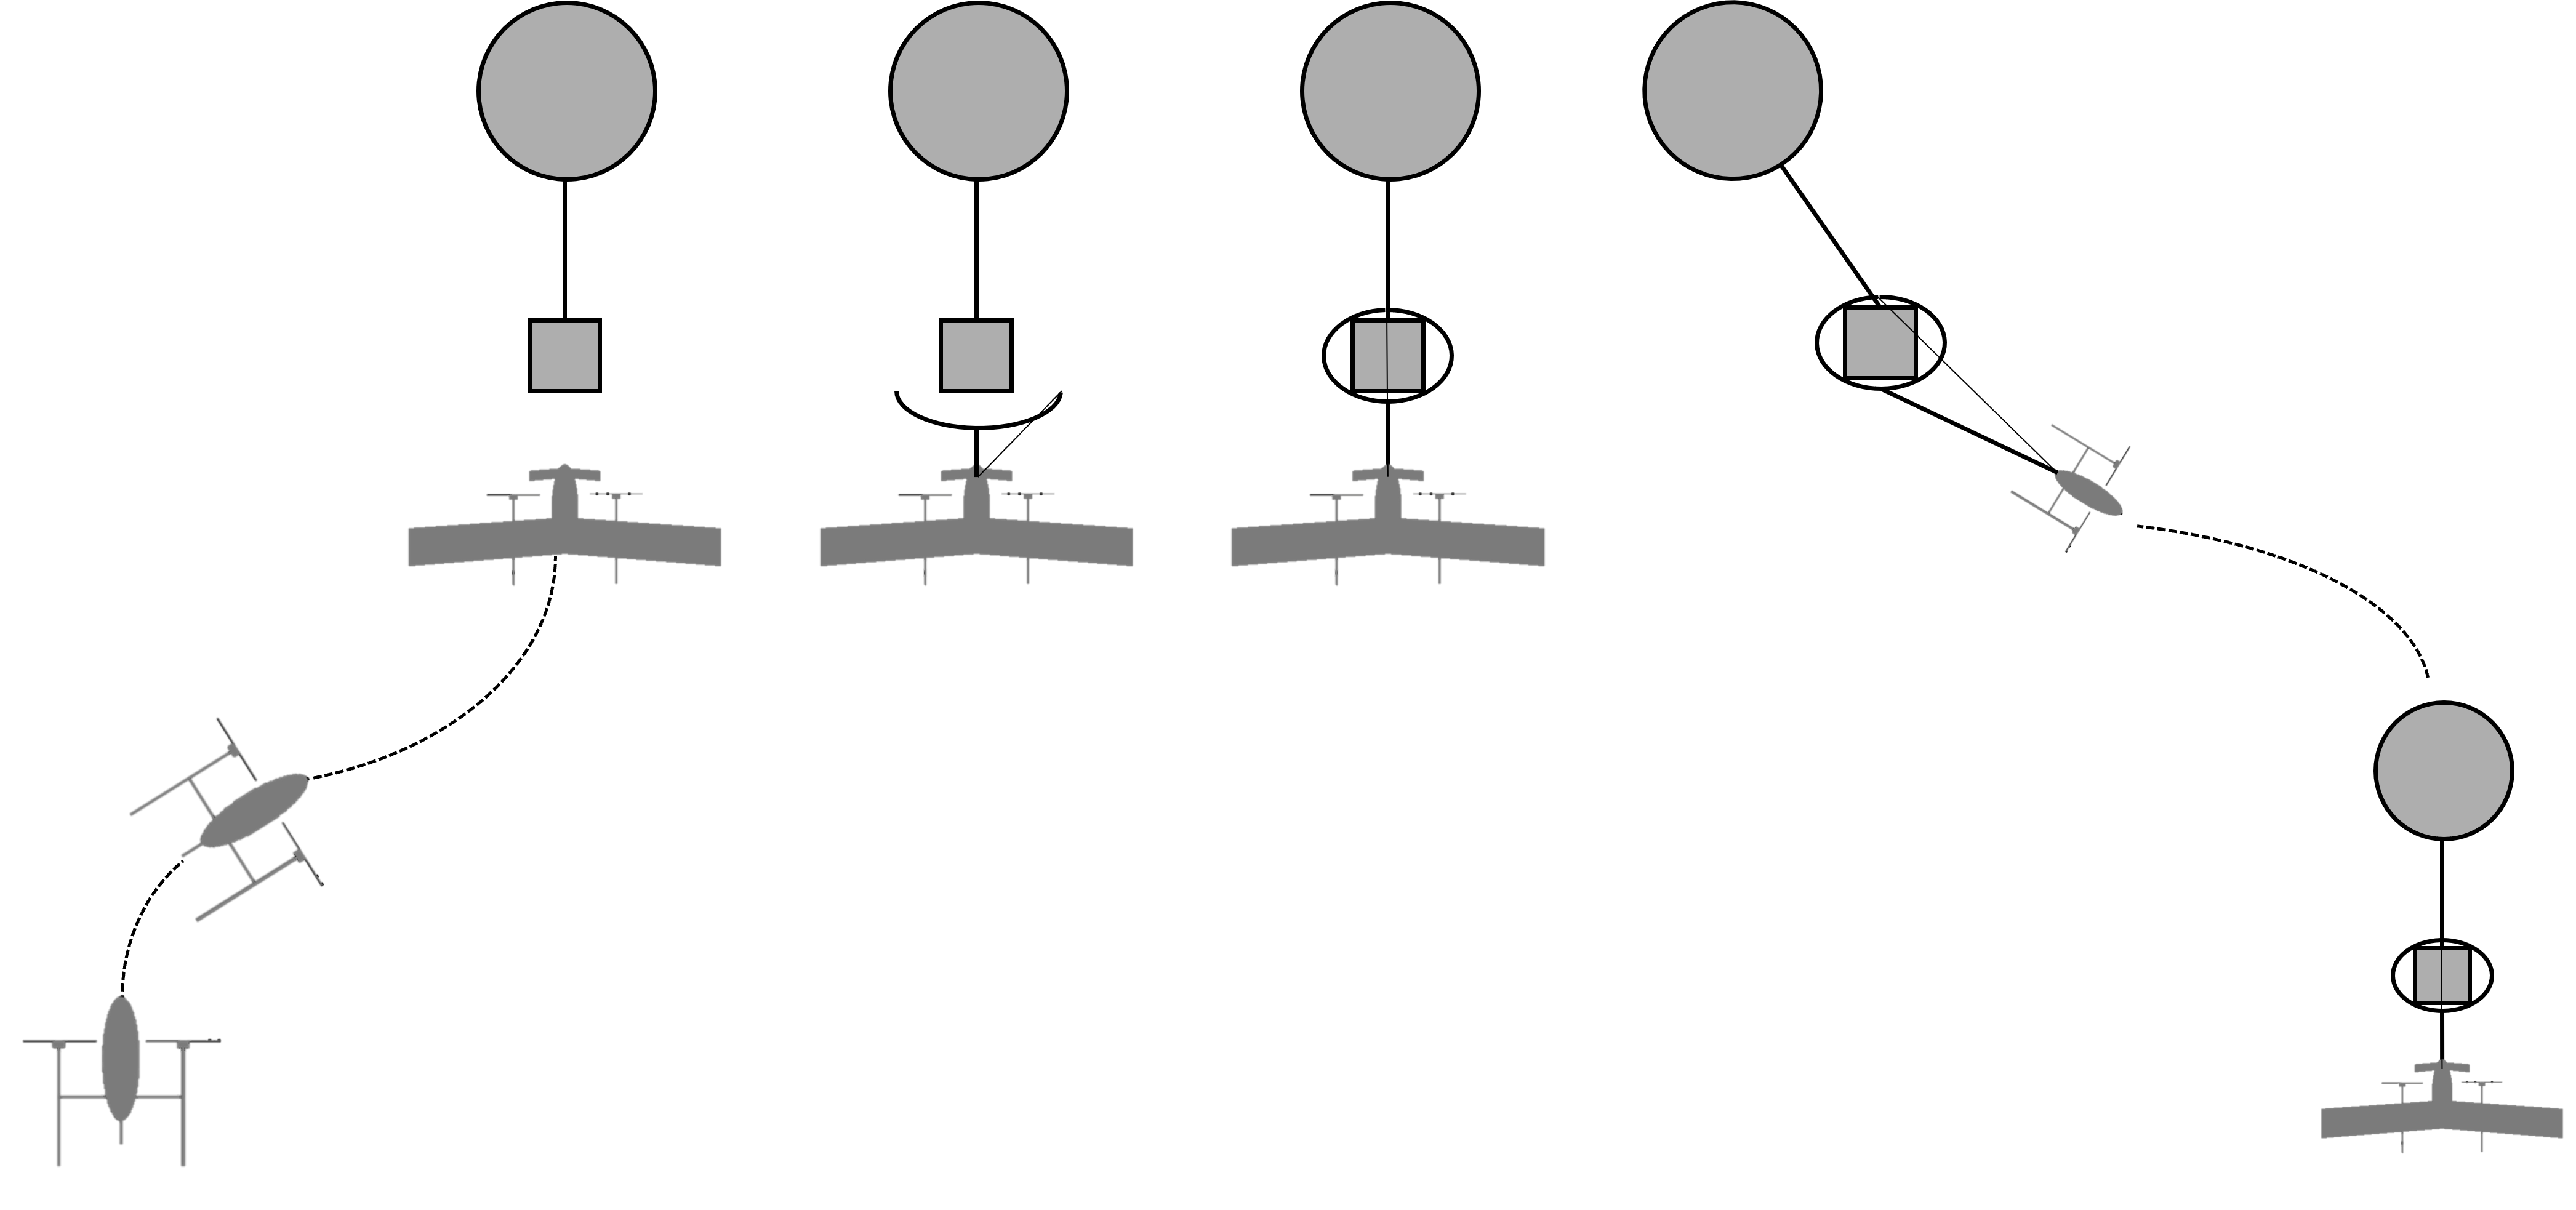
\includegraphics[width=0.7\linewidth]{figures/Concepts/Fishing - Order of Operations.png}
    \caption{Concept A - Order of Operations}
    \label{fig:CAOoO}
\end{figure}

\subsection{System Architecture}
\subsubsection{Aerial Platform}
The proposed aerial platform is a four-propeller tail-sitter UAV, as shown in \autoref{fig:ConceptADesign}. This configuration is selected because the mission requires both efficient cruise and stable hover. A pure multi-rotor would be simpler during capture but less efficient during climb and transit, while a fixed-wing aircraft would not be able to hover below the payload. 
The UAV uses a canard layout. The net gun and sensor suite are mounted in a compartment in the nose, while the reel and tether are placed near the center of mass to reduce moments during towing. 

\begin{figure}[H]
    \centering
    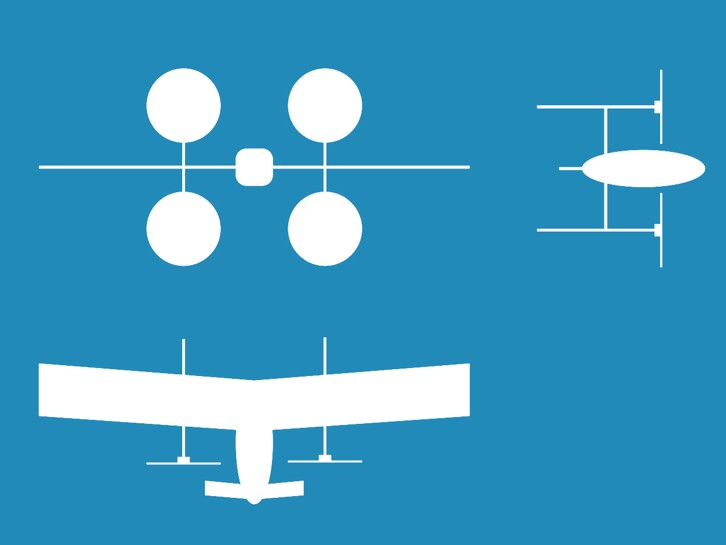
\includegraphics[width=0.4\linewidth]{figures/Concepts/Fishing Design.jpg}
    \caption{Design of Concept A}
    \label{fig:ConceptADesign}
\end{figure}

\subsubsection{Sensing and Tracking}
\label{subsec:Sensing_tracking}
The sensing architecture uses two stages. First, the UAV receives a signal from a radar-based ground segment. This provides an approximate position, altitude, and drift direction of the balloon. Once the balloon is closer to the target, it switches to onboard sensors for more precise tracking.

The proposed onboard sensors include an RGB camera, an infrared camera, as well as a short range LiDAR. The combination of these can be used for precise tracking in all relevant conditions, i.e. in varying light - and visibility levels. The onboard computer uses these inputs to estimate the relative position of the payload and maintain a stable hover below the target.

After capture, other sensors monitor the tether tension, to avoid excessive loads.

\subsubsection{Balloon Interaction Mechanism}
The UAV enters hover mode below the balloon payload. Then it shoots a 10x10m UHMWPE net upwards, using a compact net launcher, similar to the one in \autoref{fig:netlauncher}. Corner weights spread the net during launch, and help it to wrap around the payload. The net is attached to the UAV with a tether that is connected to a pouch-closure mechanism about the edges of the net, which ensures that as the UAV pulls on the tether, the net closes. 

As soon as the net is launched, the UAV begins to transition to horizontal flight, managing tension on the tether with the reel onboard the UAV. This is performed in such a way that the opening of the net is forced closed soon after it tangles about the payload, ensuring that the payload is securely attached to the UAV.


\todo{Add Sources to Images}
\begin{figure}[H]
    \centering
    \includegraphics[width=0.7\linewidth]{figures/Concepts/Net Launcher.png}
    \caption{Examples of Net Launchers}
    \label{fig:netlauncher}
\end{figure}

As an additional safety feature, the tether system includes an emergency breakaway function. If the balloon ruptures or the balloon tether fails, the tether separates from the UAV. A small parachute attached to the released tether then deploys and slows the descent of the payload-net system. This prevents unsafe descent of the entire system.

\subsubsection{Descent Initiation}
The UAV finishes its transition to horizontal flight and begins its descent towards the designated recovery location. Descent speed is managed to minimize risk of the balloon envelope rupturing or otherwise damaging the payload, while ensuring that the airspace hazard is promptly removed.

\subsubsection{Descent Management and Recovery}
The balloon is pulled downwards with a combination of thrust provided by the propellers and the weight of the UAV. The large mass of the UAV ensures that all balloon sizes covered by the requirements can be dragged downwards even in the case of UAV failure at this stage, ensuring the removal of the airspace hazard. Shortly before landing in a designated landing zone, the drone transitions to hover, so that it can set down on the ground. There, it sends a signal to ground operators. As the balloon has at most 100N of free lift at ground level, the 50kg mass of the drone is more than enough to anchor it to the ground until final recovery and processing by the operator. \todo{250N rather than 100N maybe, the citation is below, maybe calculate descent rate for a 6m balloon with 25kg of dead weight(50-25)}

\subsubsection{Ground Segment and Operator Role}
In this concept, the ground station is used primarily for long-range tracking and coordination, providing the approximate location of the balloon to the UAV via a datalink and communicating with airport or other relevant authorities to ensure safe and timely operation.




\subsection{Mass, Cost, and Complexity Estimate}

The mass and cost estimate is based on a 50 kg tail-sitter UAV carrying a net launcher, sensor package, tether reel, battery system, and propulsion system. The capture hardware is relatively light compared with the propulsion and energy storage systems. A breakdown of the cost and mass budgets can be found in \autoref{tab:budgetsA}.

\begin{table}[H]
\centering
\caption{Mass and Cost Estimates for Option A}
\label{tab:budgetsA}{%
\begin{tabular}{lll}
\hline
\textbf{Part}                                   & \textbf{Mass {[}kg{]}} & \textbf{Cost {[}€{]}} \\ \hline
Net (incl. Net, Corner Weights, and Tether)     & 2                      & 150                   \\
Net Gun                                         & 2                      & 450                   \\
Sensors (incl. Cameras, LiDAR, and Telemetry)  & 1                      & 1500                  \\
Flight Controller                               & 0.5                    & 500                   \\
Power Source (incl. Batteries and Cabeling)     & 18.2                   & 2000                  \\
Propulsion (incl. Motors, Propellers, and ESCs) & 12                     & 5000                  \\
Airframe                                        & 10                     & 3000                  \\
Miscellaneous                                   & 4.3                    & 1000                  \\
\textbf{Total}                                  & \textbf{50}            & \textbf{13 600}       \\ \hline
\end{tabular}%
}
\end{table}

More details on the aerial system can be found in \autoref{tab:SpecsA}.

\begin{table}[H]
\centering
\caption{Concept A: Specifications of Aerial System}
\label{tab:SpecsA}
\begin{tabular}{ll}
Number of Rotors         & 4                       \\
Maximum Thrust per Rotor & 35 kg                   \\
CL cruise                & 0.5                     \\
Wing Area                & 7.4m\textasciicircum{}2 \\
Battery Capacity         & 11.8 MJ                 \\ \todo{kWh bro who uses joules}
Cruise Speed             & 20 m/s                 
\end{tabular}
\end{table}

\subsection{Risks and Uncertainties}
The main risk is failed net capture. The payload may swing or have an irregular shape, leading to the net missing, and falling back down on the drone. This can be mitigated by using a large net. 

A second risk is unreliable sensing in poor visual conditions. Clouds or low-light conditions can reduce tracking performance. For this reason, multiple sensor, combining visual, depth, and ground tracking, are used.

Another important risk is sudden loss of balloon lift. If the balloon ruptures or the payload enters free fall while attached to the UAV, the tether load could destabilize the aircraft. The backup parachute reduces this risk by separating the UAV from the falling payload and slowing the payload descent.

Finally, the tail-sitter transition while carrying a tethered load is a significant control challenge. The concept therefore depends strongly on reliable hover tracking, tether-load management, and flight-control testing with representative loads.

\subsection{Summary and conclusions}
This concept provides a reliable method for recovering an uncooperative balloon. Its main strength is that it captures the payload from below without intentionally rupturing the balloon envelope. The tail-sitter UAV provides efficient transit while retaining hover capability for capture and landing.

The concept is attractive from a mass and cost perspective, with an estimated total mass of 50 kg and an estimated part cost of 13600€. The capture mechanism itself is relatively simple and light.

\section{Concept B: Pick and drop}

The system comprises three cooperating heavy-lift multirotors carrying a shared two-stage capture net (net carriers), supported by a fourth auxiliary multirotor for tether engagement and envelope intervention (intervention drone), that are delivered to the interception site by a fixed-wing carrier EVTOL. The net carriers approach the balloon-payload system from below and match its descent trajectory to establish a stable relative position. The intervention drone then ascends along the existing balloon tether and attaches a mechanical clamp at its upper end, near the balloon load ring. The clamp is connected via a Dyneema leash to an electric winch mounted on the net rim, which retracts the leash to draw the balloon and payload into proximity within the capture volume, while also closing the inner circle, like a bag, at the top of the payload. In the second stage, the outer circular net envelops the balloon and later closes it in the same manner as the inner bag. With the target fully secured, the auxiliary vehicle applies an adhesive rip-patch to the envelope to initiate  deflation, and simultaneously deploys a guided parafoil from the net rim to manage the subsequent descent.

\subsection{System Architecture}
\label{subsec:concept_B_architecture}

\subsubsection{Aerial Platform}
The capture team consists of three heavy-lift multirotor net carriers (per-vehicle MTOW 8.5 kg) plus a fourth, smaller intervention drone for tether engagement and envelope intervention. The four vehicles are packed as payload inside a fixed-wing EVTOL carrier (MTOW 81 kg at launch) that performs the climbing-cruise leg. The split between transport and capture vehicles is taken because the carrier benefits from a higher L/D value over the 6 km transit, while hover capable rotors are needed only locally.

\subsubsection{Sensing and Tracking}
Initial detection is provided by a surveillance radar on a ground station. Once the carrier is close enough to the target, the tracking is handed off to onboard EO/IR. During engagement, the intervention drone uses vision-based line-following to track the existing balloon tether for the climb.

\subsubsection{Balloon Interaction Mechanism}
A shared two-stage net (8~m diameter aperture, 50 m$^2$) is suspended horizontally between the three net carriers via burn-wire releasable suspension cables. The intervention drone delivers a mechanical clamp to the upper end of the balloon tether near the load ring; the clamp is connected through 35 m of 2 mm Dyneema leash to an electric winch on the net rim. The inner-stage drawline cinches around the payload at the top, and the outer-stage drawline cinches around the balloon. Figure~\ref{fig:net_layout} shows the flat layout, including drone attachment points D1, D2, D3 and the inner-circle dimensions.

\begin{figure}[H]
    \centering
    \includesvg[width=0.7\textwidth]{net_layout}
    \caption{Top-down view of the net flat state ($r \approx 0.97$ m inner circle).}
    \label{fig:net_layout}
\end{figure}

\subsubsection{Descent Initiation}
Descent is initiated by controlled deflation. An adhesive rip-patch (100 g, 10$\times$10 cm contact area) with embedded NiChrome burn-wire is applied through the upper net stage. The burn-wire softens the envelope material, and the intervention drone, held at 5 m standoff and still connected to the patch by a wire, pulls the patch free, opening an aperture of 0.05 m$^2$. Effusion proceeds at 0.07 kg/s for a $\varnothing$6~m helium balloon at altitude, giving a buoyancy half-life of 80 s. The envelope remains contained inside the closed net throughout deflation.

\subsubsection{Descent Management and Recovery}
A guided ram-air parafoil with an Autonomous Guidance Unit (AGU), sized for 60 kg descent mass at 5 m/s, is packed in a deployment bag tied the net rim, placed on the bottom and on the exterior of the inner payload ring so its weight distributes evenly across the three drones during transit. A spring ejection system ensures immediate canopy exposure regardless of bundle orientation; a pilot chute then extracts the main canopy, which inflates in 3 s. Three independent burn-wire cable cutters on the net-to-drone suspension cables fire simultaneously to release the captured bundle, which descends to the landing zone at 5 m/s with 30-50 m circular error.

\subsubsection{Ground Segment and Operator Role}

A  ground station provides radar surveillance, mission command, and serves as the launch and return point for the carrier and capture team. A recovery crew is dispatched to the parafoil landing zone to retrieve the net, envelope, payload and parafoil. The capture drones, intervention drone and carrier return autonomously to the ground station after the bundle is released.



% \subsection{Design Visualization}
 
% The phased deployment, moving from the ground state to full balloon envelopment, is detailed in Figure \ref{fig:deployment_sequence}.

% \begin{figure}[H]
%     \centering
%     % Swapped to be second
%     \includesvg[width=1.1\textwidth]{deployment_sequence}
%     \caption{Deployment sequence}
%     \label{fig:deployment_sequence}
% \end{figure}

\subsection{Preliminary Mass, Power and Cost Estimate}

A compact first-order sizing was performed for the split-mission Concept~B architecture. The carrier transports the three-drone capture team to $6000~\mathrm{m}$ altitude and $6000~\mathrm{m}$ ground range using wing-borne climbing cruise. The net-carrying rotorcraft are sized only for the local capture hover and powered descent after release. The sizing assumes $265~\mathrm{Wh/kg}$ batteries with $20\%$ reserve, rotor disk loading of $15~\mathrm{kg/m^2}$, rotor figure of merit $0.70$, and carrier $L/D=12$. The vehicle costs are order-of-magnitude component-scaled estimates, while payload-hardware costs are retained from the existing concept estimate.

\begin{table}[H]
\centering
\small
\caption{Hybrid carrier mass, power and cost estimate.}
\label{tab:conceptB_carrier_compact}
\begin{tabular}{lrr}
\hline
\textbf{Item} & \textbf{Mass / power} & \textbf{Cost [EUR]} \\
\hline
Structure & $20.33~\mathrm{kg}$ & $6\,100$ \\
Propulsion & $16.26~\mathrm{kg}$ & $6\,800$ \\
Avionics and control & $4.07~\mathrm{kg}$ & $5\,400$ \\
Battery & $13.17~\mathrm{kg}$ & $1\,450$ \\
Mass margin & $2.03~\mathrm{kg}$ & $500$ \\
Delivered capture-team payload & $25.45~\mathrm{kg}$ & -- \\
\hline
\textbf{Carrier MTOW / vehicle cost} & \textbf{$81.31~\mathrm{kg}$} & \textbf{$20\,000--25\,000$} \\
\hline
Loaded climbing-cruise power & $12.05~\mathrm{kW}$ & -- \\
Unloaded descent power & $2.48~\mathrm{kW}$ & -- \\
Usable battery energy & $2.79~\mathrm{kWh}$ & -- \\
\hline
\end{tabular}
\end{table}

\begin{table}[H]
\centering
\small
\caption{Single net-carrying rotorcraft mass, power and cost estimate. Three identical vehicles are used.}
\label{tab:conceptB_rotorcraft_compact}
\begin{tabular}{lrr}
\hline
\textbf{Item} & \textbf{Mass / power} & \textbf{Cost [EUR]} \\
\hline
Structure & $1.70~\mathrm{kg}$ & $500$ \\
Propulsion & $1.53~\mathrm{kg}$ & $650$ \\
Avionics and control & $0.42~\mathrm{kg}$ & $550$ \\
Battery & $0.99~\mathrm{kg}$ & $100$ \\
Mass margin & $0.18~\mathrm{kg}$ & $50$ \\
Allocated capture hardware & $3.67~\mathrm{kg}$ & -- \\
\hline
\textbf{Rotorcraft MTOW / vehicle cost} & \textbf{$8.48~\mathrm{kg}$} & \textbf{$1\,800--2\,200$} \\
\hline
Hover power & $1.26~\mathrm{kW}$ & -- \\
Powered-descent power & $0.38~\mathrm{kW}$ & -- \\
Energy requirement & $209~\mathrm{Wh}$ & -- \\
\hline
\end{tabular}
\end{table}

\begin{table}[H]
\centering
\small
\caption{Payload and capture-hardware mass and cost estimate. Values not produced by the sizing code are retained from the concept hardware estimate.}
\label{tab:conceptB_payload_compact}
\setlength{\tabcolsep}{4pt}
\begin{tabularx}{\linewidth}{lrrX}
\hline
\textbf{Element} & \textbf{Mass [kg]} & \textbf{Cost [EUR]} & \textbf{Note} \\
\hline
Capture net & $2.0$ & $2\,000--3\,000$ & HMPE/Dyneema mesh with reinforced rim \\
Main shortening/winch mechanism & $1.3$ & $1\,000--1\,500$ & Motor, drum, frame, ESC and Dyneema leash \\
Cinch drawline mechanism & $0.4$ & $200--400$ & Secondary net-closure mechanism \\
Guided parafoil with AGU & $5.0$ & $8\,000--15\,000$ & Sized for $60~\mathrm{kg}$ descent mass at $5~\mathrm{m/s}$ \\
Rip-patch and burn-wire kit & $0.5$ & $200--400$ & Controlled balloon deflation device \\
Net-to-drone release hardware & $0.3$ & $150--300$ & Three burn-wire cable cutters \\
Auxiliary intervention drone & $1.5$ & $1\,200--1\,500$ & Tether engagement and patch application \\
\hline
\textbf{Payload hardware subtotal} & \textbf{$11.0$} & \textbf{$12\,750--22\,100$} & Carried by the three net-carrying rotorcraft \\
\hline
\end{tabularx}
\end{table}

The carrier reaches the release point after approximately $600~\mathrm{s}$, matching the $10~\mathrm{min}$ reference interception time. Including the $300~\mathrm{s}$ capture hover phase, capture completion occurs after approximately $900~\mathrm{s}$. The total hardware acquisition estimate for Concept~B is therefore approximately $38\,000--54\,000$, combining the carrier, three net-carrying rotorcraft, and the payload hardware package.




 

\section{Concept C: Mechanical Cracker}

\subsection{Mission Architecture}
\noindent 
The mission architecture centers on a lift and cruise EVTOL UAV (presented in \autoref{fig:liftcruiseconcept}) that intercepts the target balloon by maneuvering into a precise station-keeping position directly beneath the payload. Once positioned, the platform deploys a pair of horizontal aluminum beams that extend outward to establish the capture frame. Through integrated actuators, these beams pivot upward to mechanically constrain and "hug" the payload, securing it firmly. Following successful capture, the system initiates a controlled descent primarily driven by gravity, utilizing its weight and high-torque thrusters to modulate airspeed and provide active stabilization. This thrust-vectoring capability ensures a managed deceleration, allowing the UAV to execute a vertical landing at a pre-designated safe recovery zone.
\begin{figure}[htbp]
     \centering
     % Right Image: The Drone Concept
     \begin{subfigure}[b]{0.56\textwidth}
    
         \centering
         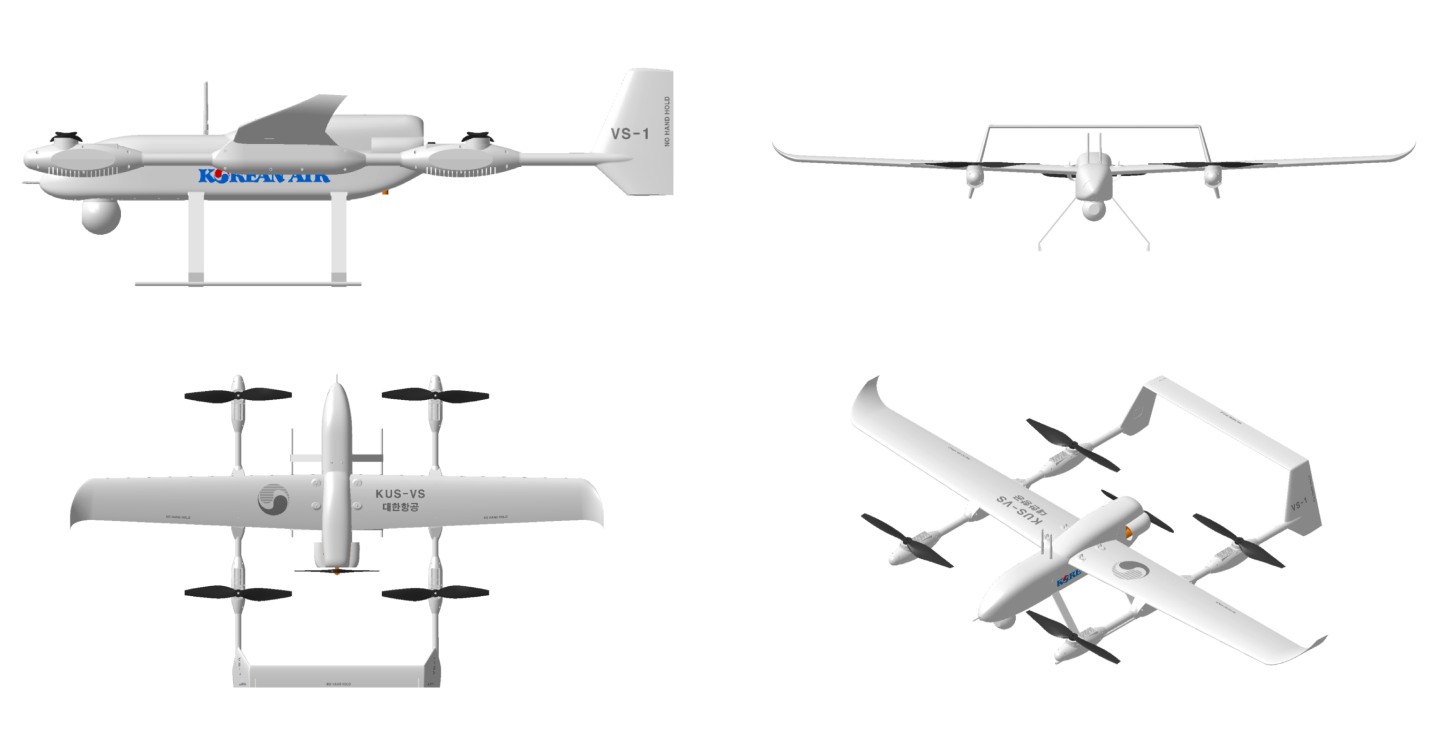
\includegraphics[width=\textwidth]{figures/Drone_concept.png}
          
         \caption{Integrated Lift \& Cruise Concept}
         \label{fig:liftcruiseconcept}
     \end{subfigure}
     \hfill
     % Left Image: The Mechanism
     \begin{subfigure}[b]{0.32\textwidth}
         \centering
         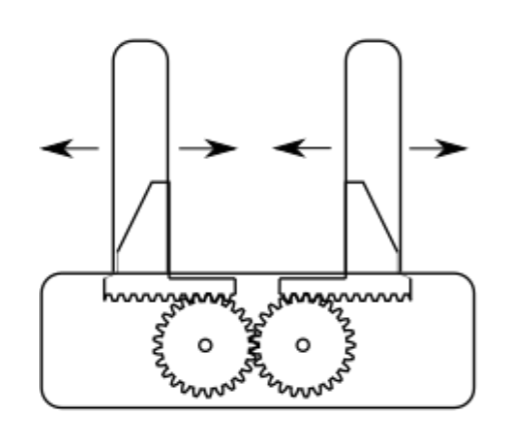
\includegraphics[width=\textwidth]{figures/Clamp_report.png}
         \caption{Linear Clamping Mechanism}
         \label{\fig:clamping_mechanism}
     \end{subfigure}
     
     \caption{From mechanical logic to aerial integration.}
     \label{fig:drone_design}
\end{figure}


\subsection{Mission phases}
\begin{enumerate}
    \item \textbf{Detection and approach} ($t < 0$). Ground radar at the mobile pickup-truck ground station hands off the target to onboard EO/IR. The response drone aparatus, launches and transits up to 6~km to the predicted intercept point. Climb rate 5~m/s, cruise speed 18--22~m/s 
    
    \item \textbf{Approach from below} ($t = 0$). The response drone places itself below the balloon-payload system, matching its drift trajectory. IT is now ready for the deployment of the Interaction Mechanism.
    
    \item \textbf{Mechanism Deployment} ($t \approx 0$ to 120~s). The system in a stationary condition allows the mechanism to be deployed. Namely, once the system detects the size of the payload, the hydraulic actuators extend and rotate 90 degrees the aluminum beams on the opposite side of the payload. Then the actuator moves one of the vertical beams towards the payload, until they tightly hold the payload. Once it is secured, the descent of the payload can begin. 
    
    
    \item \textbf{Descent and recovery} ($t > 120$~s). Using the added weight of the interception system on the balloon-payload couple, the descent commences. It descends under controlled guidance, using the drone's thrust to control the rate of descent and maneuverability in horizontal plane. It descend at a rate of $\sim$5~m/s to the designated landing zone with $\sim$30--50~m CEP. Then, the recovery crew retrieves the net, envelope, payload, and parafoil at the LZ.
\end{enumerate}


\subsection{Interaction Mechanism Conceptual Design}
The initial estimation of the interaction mechanism parameters that are important for the trade-off can be performed by the initial sizing of its elements. Due to risk of the uncontrolled balloon sheet perforation during mechanical attachment to the lifting part, it was decided that the only part to intercept safely is the payload or its attachment. According to the literature study conducted in the project Baseline Report \cite{}, different types of meteorology and smuggling balloons are characterized by different payload size, weight and securing ropes. These can be attached at various angles and to different parts of the payload, which poses a threat of cutting them with the rotor blades or having less control over them. Using the Design Option Tree presented in the same states several options to mechanically control the payload. Choosing the best option may be based on the payload type and characteristics.  \newline
Payload description \newline
The uncertainties and possibility of object geometry and package modification make the suction, adhesion, and enveloping soft gripper  methods non-adaptable to different shapes and modifications that are easy to introduce (baseline) \cite{}. Mechanisms capturing the full payload are the only feasible options left when adaptability is taken into consideration as they offer the best controllability of the balloon. 
\subsubsection{Initial sizing}
The first order estimation of the clamping mechanism is based on the configuration layout and forces expected during the deployment and descent phases. The interaction is based on the friction mechanism including strong forces between the vertical arms and the payload. Safe balloon capture that should not pose a risk to the ropes failing means that maximum downward force should not be too large. This is why, using the initial estimate of 50 kg ballast achieved by decreased drone lift which allows for the descent from 6000 meters in no more than 20 minutes using ballast and drag force calculation. This limit also ensures that the safety factor of 2.25, typically enforced for ropes by the regulatory institutions \cite{EASA2009EuropeanCS-31HB}, will not be exceeded. This means that 245 Newtons force will be exerted on the each arm of the mechanism by the balloon. Using Aluminum 6061 T6, a standard aerospace structural material, allows for the estimation of static friction coefficient to be 0.3 or more for the most of materials and can be easily increased by adding sharp edges to the structure. With that information, the normal load of $
\frac{245}{0.3}=817 \, \text{N}$ is required to sustain it. Another load is imposed by the balloon drag, which adds additional $894.4 \, \text{N}$ to the critical arm. The Free Body Diagram representing this arm with reaction forces is presented in \autoref{fig:FBD}.

\begin{figure}[h!]
    \centering
    \documentclass[tikz,border=10pt]{standalone}
\usetikzlibrary{arrows.meta, calc, patterns}

\begin{document}
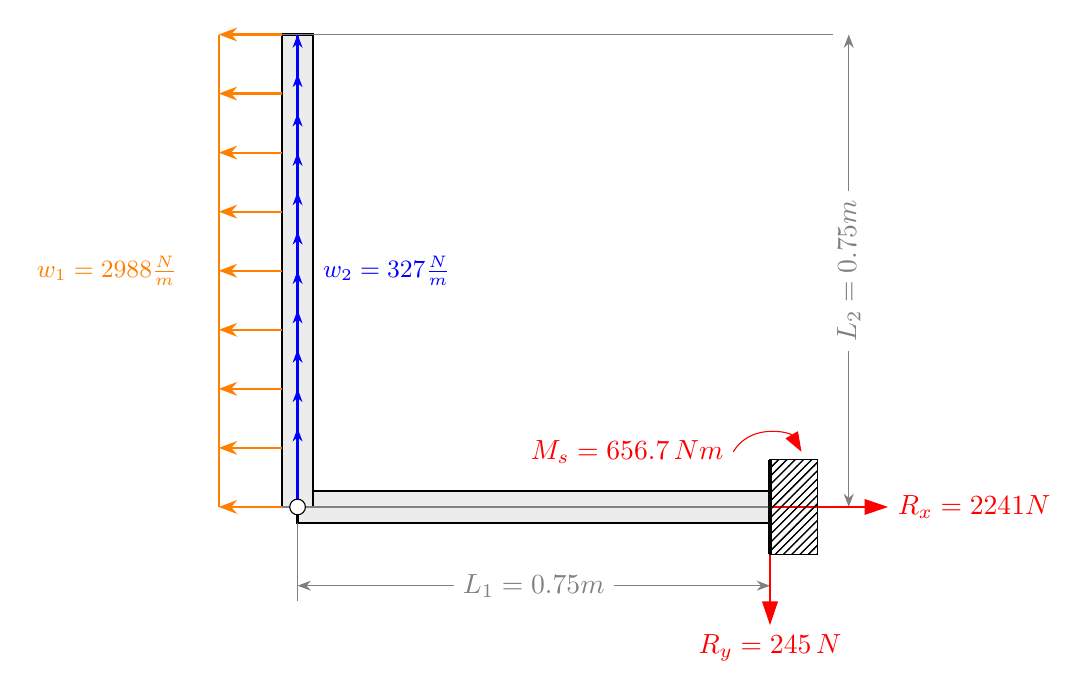
\begin{tikzpicture}[
    force/.style={- {Stealth[scale=1.2]}, red, thick},
    reaction/.style={- {Stealth[scale=1.2]}, blue!70!black, thick},
    beam/.style={draw=black, fill=gray!15, thick},
    joint/.style={circle, draw=black, fill=white, inner sep=2pt},
    ext/.style={gray, thin},
    dim/.style={<->, >=Stealth, gray, thin}
]

    % --- Parameters ---
    \def\L{6}           % Visual length
    \def\width{0.4}     % Beam thickness
    \def\loadL{4.5}     % Length of the distributed load
    \def\arrowgap{0.6}  % Number of arrows in the load

    % --- Coordinates ---
    \coordinate (Shoulder) at (0,0);
    \coordinate (Elbow) at (-\L, 0);
    \coordinate (Wrist) at (-\L, \L);

    % --- Draw Support (Fixed Shoulder) ---
    \draw[pattern=north east lines, draw=black] (0,-0.6) rectangle (0.6,0.6);
    \draw[ultra thick] (0,-0.6) -- (0,0.6);

    % --- Draw Beams ---
    \draw[beam] (-\L, -\width/2) rectangle (0, \width/2); % Beam 1
    \draw[beam] ({-\L-\width/2}, 0) rectangle ({-\L+\width/2}, \L); % Beam 2

    % --- Dimensioning for Beam 1 (Horizontal) ---
    \def\offH{-1} % Offset below the beam
    \draw[ext] (-\L, -\width/2) -- (-\L, \offH - 0.2); % Left extension
    \draw[ext] (0, -\width/2) -- (0, \offH - 0.2);      % Right extension
    \draw[dim] (-\L, \offH) -- (0, \offH) 
        node[midway, fill=white] {$L_1 = 0.75\text{m}$};

    % --- Dimensioning for Beam 2 (Vertical) ---
    % Placed further to the left to avoid your friction load
    \def\offV{7} 
    \draw[ext] ({-\L-\width/2}, 0) -- ({-\L+\offV-0.2}, 0); % Bottom extension
    \draw[ext] ({-\L-\width/2}, \L) -- ({-\L+\offV-0.2}, \L); % Top extension
    \draw[dim] ({-\L+\offV}, 0) -- ({-\L+\offV}, \L) 
        node[midway, fill=white, rotate=90] {$L_2 = 0.75\text{m}$};
        
    % --- Reaction Forces (Shoulder) ---
    % Placed clearly with arrows
    \draw [red, -{Triangle[length=3mm, width=2mm]}] (0,0) -- (1.5, 0) node[right] {$R_x = 2241 \text{N}$};
    \draw [red, -{Triangle[length=3mm, width=2mm]}] (0,0) -- (0, -1.5) node[below] {$R_y=245 \,\text{N}$};
    % Moment reaction (since it's a fixed support)
        \draw[red, {Triangle[length=2.5mm, width=1.8mm]-}] (0.4, 0.7) arc (30:150:0.5) node[left] {$M_s=656.7 \, \text{Nm}$};
    
    % --- Distributed Friction Load (Downward) ---
    % Vertical line to the left of Beam 2
    \draw[blue, thick] ({-\L}, 0) -- ({-\L}, {\L});
    \foreach \x in {0, 0.5, ..., 5} {
    \draw[blue, Stealth-] (-\L,\L-\x) -- (-\L, \L-\x-0.5);
  }
    % Label for the blue friction load positioned to the right
    \node[right, blue, font=\small, align=left] at (-\L + 0.2, \L/2) {
        $w_2 = 327 \frac{\text{N}}{\text{m}}$
    };
   % --- Distributed Normal Load (Horizontal/Perpendicular) ---
    % For a vertical beam, the normal load acts horizontally. 
    % --- Distributed Normal Load (Horizontal/Perpendicular) ---
    % Arrows now start at the beam surface and point left toward the boundary line
    \def\normL{6}      % Length of the load distribution
    \def\normX{-1}   % Horizontal offset for the load line
    
    % Boundary line for the normal load (the "tips" of the arrows)
    \draw[orange, thick] ({-\L+\normX}, \L) -- ({-\L+\normX}, {\L-\normL});
    
    % Horizontal arrows pointing LEFT
    \foreach \y in {0, 0.75, ..., \normL} {
        \draw[orange, -Stealth, thick] ({-\L-\width/2}, {\L-\y}) -- ({-\L+\normX}, {\L-\y});
    }
    
    % Label for Normal Load (moved slightly further left to avoid arrow overlap)
    \node[left, orange, font=\small, align=right] at ({-\L+\normX-0.3}, {\L-\normL/2}) {
        $w_1=2988 \frac{\text{N}}{\text{m}}$  
    };
   
    % --- Draw Support (Fixed Shoulder) ---
    \draw[pattern=north east lines, draw=black] (0,-0.6) rectangle (0.6,0.6);
    \draw[ultra thick] (0,-0.6) -- (0,0.6);

    \node[joint] at (Elbow) {};
\end{tikzpicture}
\end{document}
 % Includes the file content directly
    \caption{FBD of the critical arm}
    \label{fig:FBD}
\end{figure}
Simple structural optimization code that included rectangular thin-walled cross section of the minimum width of $0.1 \, \text{m}$ for the mechanical arms. The standard safety factor of $1.2$ is taken into account for yielding, Euler column buckling and thin sheet buckling due to bending and normal stresses.  The output of this process resulted in the $0.1 \times0.04\times0.0025 \, \text{m}$ for the critical arm counteracting the drone load and $0.14 \times0.04\times0.0025 \, \text{m}$$0.1 \times0.04\times0.0017 \, \text{m}$ for the clamping one. Their masses are $2.85 \, \text{kg}$ and $2.15 \, \text{kg}$ respectively.

This moving clamping mechanism requires actuators work. High torque rotating actuators are usually characterized by the high price and large weight. Linear actuators will then be used as the main clamping force, while the secondary actuators enabling only mechanical arm rotation will be used to extend the mechanism only before the interaction to reduce drag losses. Existing solutions that are ready to sustain the loads can weight $1-2 \, \text{kg}$ and cost up to $500$ EUR. With 2 of them being used, and conservative estimation for easier arm rotation, the mass of actuators goes up to 8 kg in total, and up to 2000 EUR.   


\begin{table}[h]
    \centering
    \caption{Mass and cost estimates for the capture hardware. Costs are 2026 EUR. Net cost reflects custom small-batch HMPE/Dyneema mesh manufacture; parafoil cost reflects guided ram-air system with autonomous guidance unit (AGU).}
    \label{tab:capture_hardware}
    \setlength{\tabcolsep}{4pt}
    \renewcommand{\arraystretch}{1.2}

    \begin{tabularx}{\linewidth}{@{}
        >{\raggedright\arraybackslash}p{0.34\linewidth}
        >{\raggedleft\arraybackslash}p{0.12\linewidth}
        >{\raggedleft\arraybackslash}p{0.15\linewidth}
        >{\raggedright\arraybackslash}X
        @{}}
        \hline
        Item & Mass [kg] & Cost [EUR] & Notes \\
        \hline
        Aluminium beams (3 meters long total)  & 5 & 150-400 & Burn-wire cable cutters, $\sim$100~g each \\
        Actuator hydraulic mechanism & 4 & 800-1000 & Electric winch, smaller than main retraction unit \\
        Second Actuator hydraulic mechanism & 4 & 800-1000 & Electric winch, smaller than main retraction unit \\
        \hline
        \textbf{Capture hardware subtotal} & \textbf{13} & \textbf{1\,750-2\,400} & Distributed across the 3-drone formation \\
        \hline
    \end{tabularx}
\end{table}

\subsection{Aerial Platform Selection}

When performing the platform trade-off for the intercepting UAV, several critical factors must be evaluated. The primary requirement is the ability to maintain stable level flight and interact precisely with the balloon-payload system. This necessitates robust control laws capable of managing high-altitude atmospheric conditions and executing complex maneuvers.

Reliability is the second key priority, focusing on system robustness to ensure consistent performance, prevent mid-air failures, and minimize long-term maintenance costs. Cost follows as the third most significant criterion; procurement, manufacturing, and integration expenses must remain strictly within the allocated budget.

Furthermore, safety and regulatory compliance are mandatory to mitigate risks to third parties and ensure adherence to international Unmanned Aircraft System (UAS) airspace regulations. Finally, sustainability is addressed by evaluating the environmental impact of the UAV's lifecycle and prioritizing energy-efficient propulsion to ensure ecologically responsible deployment.

In light of these criteria, the aerial platforms identified in the Baseline Report (\todo{reference}) were evaluated. Due to the requirement for hovering during the approach and grasping of the payload, the fixed-wing concept was eliminated. Tilt-rotor and tailsitter configurations were also dismissed due to their inherent mechanical and control complexity. Between the remaining options—multirotor and lift-and-cruise configurations—the latter was selected for its superior precision and control capabilities during the interception phase.

\subsection{Preliminary Mass, Power and Cost Estimate}

A preliminary Mass, Power sizing is perfromed for the proposed UAS system.  It has been perfromed using the same structre as in the previous section ( ref it), where the payload mass comes ot 13 kg, the total MTOW is 69 kg, with a 22.5 kg battery mass delivering 3.96 kWh of energy available. 

\begin{table}[H]
    \centering
    \caption{Preliminary mass and power estimate for the hybrid  UAS system.}
    \label{tab:carrier_sizing}
    \begin{tabular}{lr}
        \hline
        Parameter & Estimate \\
        \hline
        Delivered payload mass & $13~\mathrm{kg}$ \\
        Carrier MTOW at launch & $69~\mathrm{kg}$ \\
        Battery mass & $22.5~\mathrm{kg}$ \\
        Structure mass & $19.33~\mathrm{kg}$ \\
        Propulsion mass & $11~\mathrm{kg}$ \\
        Avionics mass & $1~\mathrm{kg}$ \\
        Mass margin & $1.84~\mathrm{kg}$ \\
        Climb power & $11.39~\mathrm{kW}$ \\
        Cruise power & $1.2~\mathrm{kW}$ \\
        Descent power, unloaded & $4~\mathrm{kW}$ \\
        Hover power & $10.3~\mathrm{kW}$\\
        Usable battery energy & $3.96~\mathrm{kWh}$ \\
        Estimated rotor radius & $0.42~\mathrm{m}$ \\
        \hline
    \end{tabular}
\end{table}



\subsection{Key Risks}

\begin{table}[H]
\centering
\small
\caption{Key risks for the Mechanical Cracker concept.}
\label{tab:conceptD_key_risks}
\begin{tabularx}{\textwidth}{p{0.27\textwidth} X p{0.30\textwidth}}
\toprule
\textbf{Risk} & \textbf{Effect on mission} & \textbf{Possible mitigation} \\
\midrule
Payload has irregular shape  & UAVs cannot reliably catch the payload in a secure position & Add complexity, additional actuators and smaller parts to accommodate for irregular shapes\\
Loss of lift in  balloon & Loos of control as drone unable to carry bi payload  & Increase Thurst and slow the paylaod-balloon system to control it better, have a backup parachute for easing the drone . \\
Loss of thrust  & UAVs may lose control or the payload may swing unpredictably. & Diminish  thrust on other rotors or shut off and deploy an emergency parachute to glide down to the landing zone \\
Payload damage & Payload may be damaged by the grabbing mechanism. & Grabbing the payload at a slower pace to avoid damage. \\
Drone damage & The system may be damaged during interaction with the payload. & Increase controllability, allow for multiple attempts, and perform maneuvers slower \\

\bottomrule
\end{tabularx}
\end{table}




\section{Concept D: Cooperative Variable-Weight Payload Net}

% \subsection{Introduction}



\subsection{Introduction}

Concept D uses three cooperative multirotor UAVs to carry a shared payload-capture net. The system captures the suspended payload or lower flight train from below, instead of enclosing and deflating the full balloon envelope. After capture, the added mass of the net, ballast, tethers, and closure hardware overcomes the residual free lift of the balloon and initiates a controlled descent.

The three UAVs fly in a triangular formation and suspend the net using long tethers. This geometry keeps the rotors away from the payload, balloon tether, and possible swing envelope, while still allowing the UAVs to apply steering forces during descent. The recovery team is cued by the ground segment and uses onboard EO/IR sensing for terminal tracking and payload alignment.

\begin{figure}[H]
    \centering
    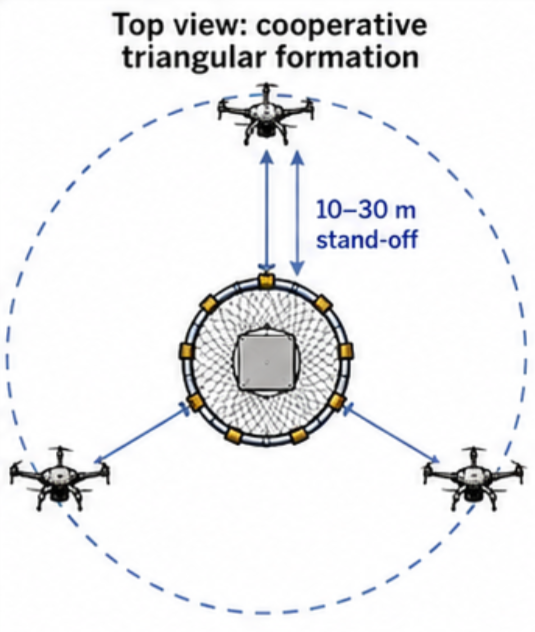
\includegraphics[width=0.35\textwidth]{figures/Concepts/conceptDtopview.png}
    \caption{Top-view conceptual layout of Concept D. Three cooperative UAVs remain connected to the payload-capture net through long tethers, allowing the formation to stabilise and steer the captured payload-net system during descent.}
    \label{fig:conceptD_topview}
\end{figure}

The interaction mechanism consists of a flexible HMPE/Dyneema payload net, a drawline closure system, distributed ballast modules, UAV-to-net tethers, and an optional backup parachute or parafoil. The net closes around the payload like a bag and mechanically locks after capture. The ballast is distributed around the net rim or lower net structure so that descent authority can be adjusted and partially released before landing.





% Concept D uses three cooperative multirotor UAVs to carry and control a shared payload-capture net. The net captures the suspended payload or lower flight train, rather than enclosing the full balloon envelope. The balloon remains intact above the captured payload, while the added mass of the net, ballast, tethers, and closure hardware increases the effective suspended weight and initiates descent.

% The UAVs approach from below in a triangular formation and suspend the capture net using long tethers. Once the payload enters the capture volume, the net closes around it and mechanically locks. Distributed ballast pouches, filled with sand or another granulated material, are integrated into the net rim or lower net structure. The ballast provides the additional downward force required to overcome the residual free lift of the balloon-payload system.

% During descent, the UAVs remain connected to the net through long tethers. Their main role is to stabilise the captured system, reduce lateral drift, and apply horizontal steering forces toward a designated recovery zone. The UAVs are therefore not intended to carry the full vertical load continuously after capture. If the descent rate becomes excessive, or if the UAVs must detach, a backup parachute or parafoil can be deployed from the net rim.

% The concept prioritises non-destructive payload capture and avoids direct interaction with the balloon envelope. Its main feasibility driver is the ballast mass required to overcome the remaining free lift of the balloon.



% \begin{figure}[H]
%     \centering
%     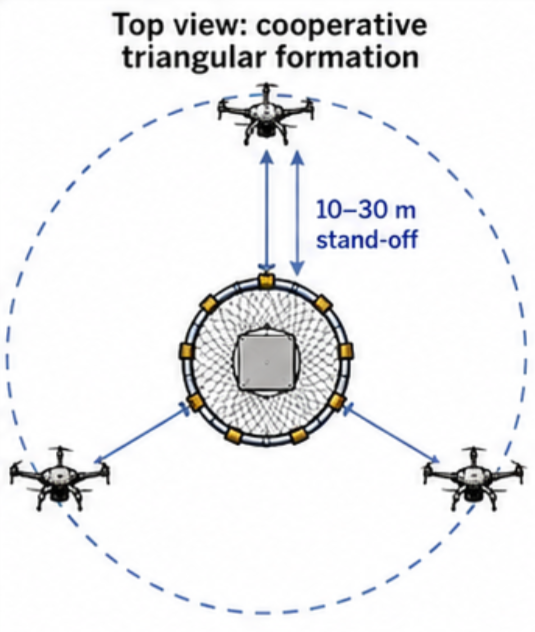
\includegraphics[width=0.35\textwidth]{figures/Concepts/conceptDtopview.png}
%     \caption{Top-view conceptual layout of Concept D. Three cooperative UAVs remain connected to the payload-capture net through long tethers, allowing the formation to stabilise and steer the captured payload-net system during descent.}
%     \label{fig:conceptD_topview}
% \end{figure}


% The top-view layout of the cooperative variable-weight payload net is shown in Figure~\ref{fig:conceptD_topview}. The three UAVs form a triangular configuration around the capture net, which provides geometric stability and allows horizontal steering forces to be applied through the tethers during descent. 


\subsection{System Architecture}
\label{subsec:concept_D_architecture}

\subsubsection{Aerial Platform}

The aerial platform consists of three coordinated heavy-lift multirotor UAVs. The UAVs climb to the interception region, form a triangular formation below the target, and carry the payload-capture net through long stand-off tethers. A multirotor configuration is selected because the concept requires accurate hover, low-speed manoeuvring, and station keeping during payload capture.

\subsubsection{Sensing and Tracking}

Initial target cueing is provided by the ground segment using radar, visual observation, or another external monitoring source. Once the UAV team reaches the search region, onboard EO/IR sensing is used for terminal tracking, payload localisation, and formation alignment below the balloon-payload system.

\subsubsection{Balloon Interaction Mechanism}

The interaction mechanism consists of a flexible HMPE/Dyneema payload-capture net, a drawline closure system, distributed ballast modules, UAV-to-net tethers, and emergency release hardware. The net is positioned below the payload and then closed around it like a bag. A mechanical lock prevents reopening after capture. The system captures the payload or lower flight train rather than the balloon envelope itself, reducing the risk of uncontrolled rupture.

\subsubsection{Descent Initiation}

Descent is initiated by adding mass to the balloon-payload system. The attached net, ballast, tethers, and closure hardware must exceed the balloon residual free lift with sufficient margin:

\begin{equation}
    \left(m_{\mathrm{net}} + m_{\mathrm{ballast}} + m_{\mathrm{hardware}}\right)g 
    >
    B_{\mathrm{balloon}} - W_{\mathrm{payload}} + F_{\mathrm{margin}}
    \label{eq:ballast_descent_condition}
\end{equation}

where \(m_{\mathrm{net}}\) is the capture-net mass, \(m_{\mathrm{ballast}}\) is the ballast mass, \(m_{\mathrm{hardware}}\) includes tethers, closure devices, and release hardware, \(B_{\mathrm{balloon}}\) is the balloon buoyancy, \(W_{\mathrm{payload}}\) is the payload weight, and \(F_{\mathrm{margin}}\) is the required descent margin.

\subsubsection{Descent Management and Recovery}

During descent, the UAVs remain connected through long tethers and provide lateral steering toward the recovery zone. The descent rate is controlled mainly through the amount of ballast attached to the net. If the descent rate becomes too high near the ground, ballast can be released gradually. If tether loads become excessive or formation control is lost, an emergency parachute or parafoil can be deployed.

\subsubsection{Ground Segment and Operator Role}

The ground station provides target cueing, mission approval, and recovery-zone coordination. It also acts as the launch and return location for the UAV team. After landing, the recovery crew retrieves the payload, net, ballast container, and reusable hardware.





\subsection{Preliminary Mass and Cost Estimate}


% \subsection{Preliminary Mass, Cost, Power and Time Estimate}

% A first-order mass, power, and time estimate was made to assess whether Concept D is feasible as a direct-climb high-altitude interception concept. The estimate is intended for trade-off comparison, not final propulsion sizing.

% For the capture system, the attached mass is driven by the residual free lift of the balloon rather than the full payload mass. For preliminary sizing, the attached net and ballast system is taken as approximately \(15\)--\(30\%\) of the payload mass for nominal cases, and up to \(30\)--\(50\%\) for poorly characterised targets. For a \(50~\mathrm{kg}\) payload, this corresponds to approximately \(7\)--\(15~\mathrm{kg}\) in the nominal case and up to \(25~\mathrm{kg}\) in the conservative case.


The cost estimate is based on catalogue-level component references and should therefore be interpreted as a prototype-level estimate, not a final procurement quotation. Commercial HMPE/Dyneema netting is available at low material cost, with one 4.2~m by 31~m HMPE/Dyneema netting example listed at 2.8~kg and approximately EUR~111 \cite{Netmark2026HMPE/DyneemaHM}. Dyneema tether line is also relatively low-cost, with 2~mm, 50~m line listed at approximately EUR~27--32 depending on VAT treatment \cite{Spearfishing.de2026DyneemaM}. The cinch mechanism cost is based on small servo/winch hardware, with one high-torque servo winch listed at approximately EUR~121 \cite{FlashRC2026ServoTurns}. The largest uncertainty is the backup parachute system: small certified drone parachute kits can already cost around EUR~1600, while a commercial parachute system for drones up to 25~kg is listed at USD~4499.95 \cite{MegaDron2026MOCSeries,UAVSystemsInternational2026DroneKg}. Therefore, the parachute/recovery-system cost range is intentionally broad.
\setlength{\tabcolsep}{3pt}
\renewcommand{\arraystretch}{1.25}

\begin{longtable}{@{}
    >{\raggedright\arraybackslash}p{0.23\textwidth}
    >{\raggedright\arraybackslash}p{0.11\textwidth}
    >{\raggedright\arraybackslash}p{0.13\textwidth}
    >{\raggedright\arraybackslash}p{0.46\textwidth}
@{}}

\caption{Preliminary mass and cost estimate for the Concept D payload-capture hardware. Values exclude the three UAV platforms, onboard sensing hardware, batteries, and ground equipment.}
\label{tab:conceptD_sizing_cost}\\

\toprule
\textbf{Item} & \textbf{Mass} & \textbf{Cost [EUR]} & \textbf{Basis / design relevance} \\
\midrule
\endfirsthead

\caption[]{Preliminary mass and cost estimate for the Concept D payload-capture hardware. Continued.}\\
\toprule
\textbf{Item} & \textbf{Mass} & \textbf{Cost [EUR]} & \textbf{Basis / design relevance} \\
\midrule
\endhead

\bottomrule
\endfoot

Payload capture net 
& 2-5 kg 
& 300-1500 
& HMPE/Dyneema netting with reinforced rim and custom stitching. Catalogue netting is cheaper, but custom reinforcement and integration drive the estimate \cite{Netmark2026HMPE/DyneemaHM}. \\

Tethers and attachments 
& 0.3-1.0 kg 
& 100-250 
& Dyneema tether line, knots/splices, carabiners, and UAV-to-net attachment hardware \cite{Spearfishing.de2026DyneemaM}. \\

Cinch and locking mechanism 
& 0.5-1.5 kg 
& 300-800 
& Servo/winch, drum, guide rings, locking element, ESC/driver, and structural bracket. Catalogue servo-winch hardware gives the lower-bound reference \cite{FlashRC2026ServoTurns}. \\

Granulated or liquid ballast modules 
& 5-25 kg 
& 50-300 
& Sand, water, or another low-cost ballast plus pouches/containers. Cost is low, but mass is a major feasibility driver. \\

Ballast and emergency release hardware 
& 0.8--2.3 kg 
& 300--900 
& Release valves, cutters, small actuators, wiring, and redundant emergency release links. \\

Backup parachute system 
& 1-4 kg 
& 1000-5000 
& Emergency descent-rate reduction. The range covers simple prototype parachutes up to commercial UAV recovery systems \cite{MegaDron2026MOCSeries,UAVSystemsInternational2026DroneKg}. \\

\midrule
\textbf{Subtotal with backup parachute} 
& \textbf{9.6-38.8 kg} 
& \textbf{2050-8750} 
& Prototype-level range for Concept D capture and descent hardware. \\

\end{longtable}

% For the climb-power estimate, the three UAVs are assumed to jointly carry a maximum Concept-D payload of \(30~\mathrm{kg}\), giving \(10~\mathrm{kg}\) per UAV. A fixed non-battery mass of \(22~\mathrm{kg}\) per UAV is assumed, consisting of \(12~\mathrm{kg}\) vehicle mass and \(10~\mathrm{kg}\) payload share.

% The closest publicly available heavy-lift multirotor reference is the DJI FlyCart 30. It can carry a \(30~\mathrm{kg}\) payload in dual-battery mode and lists a maximum ascent speed of \(5~\mathrm{m/s}\) with this payload under zero-altitude, windless test conditions \cite{DJI2026DJISpecifications}. However, its \(6000~\mathrm{m}\) maximum flight altitude is listed only for the no-payload case, so a loaded climb to \(6000~\mathrm{m}\) is already an optimistic assumption \cite{DJI2026DJISpecifications}. A \(10~\mathrm{m/s}\) climb rate is therefore rejected for Concept D sizing, even though smaller enterprise UAVs can reach this value with much lower payload capacity \cite{DJI2026DJISpecificationsd}. Multirotor power-consumption studies also show that vertical-ascent power is higher than hover power and increases with ascent speed \cite{Gong2022ModellingUAVs}.

% The battery sizing uses a source-anchored power-loading method. From the DJI FlyCart 30 battery energy and hover endurance, the sea-level hover benchmark is approximately \(139~\mathrm{W/kg}\). To account for vertical climb, reduced air density at \(6000~\mathrm{m}\), suspended hardware, and preliminary uncertainty, the Concept D average climb power loading is set to \(230~\mathrm{W/kg}\). A \(3~\mathrm{min}\) terminal hover/capture allowance, \(10\%\) energy contingency, and \(20\%\) unusable battery reserve are included.

% \begin{table}[H]
% \centering
% \small
% \caption{Concept D battery-mass estimate for a \(5~\mathrm{m/s}\) climb to \(6000~\mathrm{m}\), including \(3~\mathrm{min}\) terminal hover, \(10\%\) energy contingency, and \(20\%\) battery reserve.}
% \label{tab:conceptD_battery_mass_estimate}
% \setlength{\tabcolsep}{5pt}
% \renewcommand{\arraystretch}{1.15}
% \begin{tabular}{lccccc}
% \toprule
% \textbf{Battery specific} 
% & \textbf{Battery} 
% & \textbf{MTOW} 
% & \textbf{Avg. climb} 
% & \textbf{Usable energy} 
% & \textbf{Team battery} \\
% \textbf{energy} 
% & \textbf{per UAV} 
% & \textbf{per UAV} 
% & \textbf{power per UAV} 
% & \textbf{per UAV} 
% & \textbf{mass} \\
% \midrule
% \(176~\mathrm{Wh/kg}\) & \(45.3~\mathrm{kg}\) & \(67.3~\mathrm{kg}\) & \(15.5~\mathrm{kW}\) & \(6.38~\mathrm{kWh}\) & \(135.9~\mathrm{kg}\) \\
% \(220~\mathrm{Wh/kg}\) & \(25.7~\mathrm{kg}\) & \(47.7~\mathrm{kg}\) & \(11.0~\mathrm{kW}\) & \(4.52~\mathrm{kWh}\) & \(77.0~\mathrm{kg}\) \\
% \(265~\mathrm{Wh/kg}\) & \(17.8~\mathrm{kg}\) & \(39.8~\mathrm{kg}\) & \(9.15~\mathrm{kW}\) & \(3.77~\mathrm{kWh}\) & \(53.4~\mathrm{kg}\) \\
% \bottomrule
% \end{tabular}
% \end{table}

% The \(176~\mathrm{Wh/kg}\) case is close to the DJI DB2000 pack level and makes the direct-climb version impractical. Even with the optimistic \(265~\mathrm{Wh/kg}\) case, the team requires approximately \(53~\mathrm{kg}\) of batteries, \(27.5~\mathrm{kW}\) average climb power, and \(11.3~\mathrm{kWh}\) usable energy for climb and terminal capture. The climb alone takes \(20~\mathrm{min}\), so Concept D cannot meet a strict \(10~\mathrm{min}\) ground-to-intercept requirement at \(6000~\mathrm{m}\).

As a commercial off-the-shelf reference, the DJI FlyCart 30 gives an indicative purchase price for a heavy-lift UAV in this class. Public European listings place the base FlyCart 30 at approximately \(18{,}600~\mathrm{EUR}\), while more complete packages including key operating hardware are listed at approximately \(23{,}000{-}26{,}000~\mathrm{EUR}\) per UAV \cite{Copters2026FlyCart30,DigitalAgro2026FlyCart30}. For a three-UAV Concept D architecture, this would correspond to roughly \(69{,}000{-}77{,}000~\mathrm{EUR}\) for the aircraft purchase alone, excluding mission-specific nets, tethers, recovery hardware, integration, testing, spares, and additional batteries. This value should therefore be interpreted as an off-the-shelf procurement benchmark rather than the expected final production cost. A custom UAV developed from selected components would likely reduce the recurring unit cost, but would require substantially more design, manufacturing, integration, verification, and testing effort, increasing development time and project resource demand.



For the climb-power estimate, the three UAVs are assumed to jointly carry a maximum Concept-D payload of \(30~\mathrm{kg}\), giving \(10~\mathrm{kg}\) per UAV. A fixed non-battery mass of \(22~\mathrm{kg}\) per UAV is assumed, consisting of \(12~\mathrm{kg}\) vehicle mass and \(10~\mathrm{kg}\) payload share. The refined battery sizing gives a battery mass of \(19.79~\mathrm{kg}\) per UAV, resulting in an estimated MTOW of \(41.79~\mathrm{kg}\) per UAV.

The closest publicly available heavy-lift multirotor reference is the DJI FlyCart 30. It can carry a \(30~\mathrm{kg}\) payload in dual-battery mode and lists a maximum ascent speed of \(5~\mathrm{m/s}\) with this payload under zero-altitude, windless test conditions \cite{DJI2026DJISpecifications}. However, its \(6000~\mathrm{m}\) maximum flight altitude is listed only for the no-payload case, so a loaded climb to \(6000~\mathrm{m}\) is already an optimistic assumption \cite{DJI2026DJISpecifications}. A \(10~\mathrm{m/s}\) climb rate is therefore rejected for Concept D sizing, even though smaller enterprise UAVs can reach this value with much lower payload capacity \cite{DJI2026DJISpecificationsd}. Multirotor power-consumption studies also show that vertical-ascent power is higher than hover power and increases with ascent speed \cite{Gong2022ModellingUAVs}.

The battery sizing uses a source-anchored power-loading method. From the DJI FlyCart 30 battery energy and hover endurance, the sea-level hover benchmark is approximately \(139~\mathrm{W/kg}\). To account for vertical climb, reduced air density at \(6000~\mathrm{m}\), suspended hardware, and preliminary uncertainty, the refined Concept D estimate uses an average climb power of \(8.63~\mathrm{kW}\) per UAV, corresponding to approximately \(206~\mathrm{W/kg}\) on the estimated MTOW. The resulting mission energy consumption is \(3.48~\mathrm{kWh}\) per UAV, including the \(3~\mathrm{min}\) terminal hover/capture allowance and \(10\%\) energy contingency. With a \(20\%\) unusable battery reserve, the installed battery energy is \(4.35~\mathrm{kWh}\) per UAV. Using a battery specific energy of \(220~\mathrm{Wh/kg}\), this gives a required battery mass of \(19.79~\mathrm{kg}\) per UAV.


\begin{table}[H]
\centering
\small
\caption{Concept D battery-mass estimate for a \(5~\mathrm{m/s}\) climb to \(6000~\mathrm{m}\), including \(3~\mathrm{min}\) terminal hover, \(10\%\) energy contingency, and \(20\%\) battery reserve.}
\label{tab:conceptD_battery_mass_estimate}
\setlength{\tabcolsep}{5pt}
\renewcommand{\arraystretch}{1.15}
\begin{tabular}{lcccccc}
\toprule
\textbf{Battery specific} 
& \textbf{Battery} 
& \textbf{MTOW} 
& \textbf{Avg. climb} 
& \textbf{Mission energy} 
& \textbf{Installed battery} 
& \textbf{Team battery} \\
\textbf{energy} 
& \textbf{per UAV} 
& \textbf{per UAV} 
& \textbf{power per UAV} 
& \textbf{per UAV} 
& \textbf{energy per UAV} 
& \textbf{mass} \\
\midrule
\(220~\mathrm{Wh/kg}\) 
& \(19.79~\mathrm{kg}\) 
& \(41.79~\mathrm{kg}\) 
& \(8.63~\mathrm{kW}\) 
& \(3.48~\mathrm{kWh}\) 
& \(4.35~\mathrm{kWh}\) 
& \(59.37~\mathrm{kg}\) \\
\bottomrule
\end{tabular}
\end{table}




The descent estimate reuses the balloon drag method introduced in the baseline sizing section. The descent rate depends on the excess downward mass after the balloon residual free lift has been overcome.

\begin{table}[H]
\centering
\small
\caption{Indicative descent-rate and descent-time estimate after capture. \(m_{\mathrm{excess}}\) is the downward mass remaining after the balloon residual free lift has been overcome.}
\label{tab:conceptD_descent_time_estimate}
\begin{tabularx}{\textwidth}{p{0.16\textwidth} p{0.18\textwidth} p{0.18\textwidth} p{0.18\textwidth} X}
\toprule
\textbf{Balloon diameter}
& \textbf{Excess downward mass}
& \textbf{Descent rate at 6 km}
& \textbf{Descent rate near ground}
& \textbf{Approx. descent time from 6 km} \\
\midrule
\(2~\mathrm{m}\) & \(10~\mathrm{kg}\) & \(14.2~\mathrm{m/s}\) & \(10.4~\mathrm{m/s}\) & \(8.1~\mathrm{min}\). Too fast without drag augmentation or ballast release. \\
\(4~\mathrm{m}\) & \(10~\mathrm{kg}\) & \(7.1~\mathrm{m/s}\) & \(5.2~\mathrm{m/s}\) & \(16.3~\mathrm{min}\). Reasonable but still requires landing-rate control. \\
\(6~\mathrm{m}\) & \(10~\mathrm{kg}\) & \(4.7~\mathrm{m/s}\) & \(3.5~\mathrm{m/s}\) & \(24.4~\mathrm{min}\). Safe but slow; drift distance may be large. \\
\(6~\mathrm{m}\) & \(15~\mathrm{kg}\) & \(5.8~\mathrm{m/s}\) & \(4.3~\mathrm{m/s}\) & \(19.9~\mathrm{min}\). Better time budget, but requires more carried ballast. \\
\bottomrule
\end{tabularx}
\end{table}
\todo{dont put this into this section, put upstairs}

The approximate direct-climb time budget is \(20~\mathrm{min}\) for climb, \(3~\mathrm{min}\) for terminal formation and capture, and \(20\)--\(24~\mathrm{min}\) for descent of a \(6~\mathrm{m}\) balloon depending on the excess downward mass. Horizontal transit is not included because climb and translation may occur simultaneously; if performed sequentially, a \(6~\mathrm{km}\) horizontal transit at \(15~\mathrm{m/s}\) adds approximately \(6.7~\mathrm{min}\).

Overall, Concept D is attractive because it avoids destructive balloon-envelope interaction, but it is weak as a direct high-altitude interception architecture. It should be penalised in the trade-off unless combined with a carrier aircraft, pre-positioned airborne loiter, or a lower operational altitude envelope.



%\subsection{Trade-off Criteria Analysis}

%Concept D performs well in \textbf{safety} because it avoids direct destructive interaction with the balloon envelope. The main safety concerns are ballast release, descent-path prediction, tether loads, and hard landing risk.

%For \textbf{intercept capability}, the payload net is more tolerant than a rigid gripper but less tolerant than a full balloon-enclosure net. The main weaknesses are payload swing, tether length uncertainty, wind disturbance, and the long direct-climb time to \(6000~\mathrm{m}\).

%For \textbf{reliability}, the concept avoids complex deflation hardware but introduces cooperative flight, tether management, net closure, ballast release, and optional backup parachute deployment. These interacting subsystems make the concept operationally complex.

%For \textbf{cost}, the capture hardware itself is moderate, but the requirement for three heavy-lift UAVs and large battery capacity increases total system cost. For \textbf{sustainability}, the concept avoids balloon fragmentation and recovers the main hardware, but released ballast must be environmentally acceptable and restricted to the recovery zone.



\subsection{Risks and Uncertainties}

\begin{table}[H]
\centering
\small
\caption{Key risks for the cooperative variable-weight payload net concept.}
\label{tab:conceptD_key_risks}
\begin{tabularx}{\textwidth}{p{0.27\textwidth} X p{0.30\textwidth}}
\toprule
\textbf{Risk} & \textbf{Effect on mission} & \textbf{Possible mitigation} \\
\midrule
Required ballast mass is too high & UAVs cannot carry or control the net, making the concept infeasible for high-buoyancy targets. & Include a go/no-go check based on estimated residual free lift. \\
Battery mass is too high & Direct climb to \(6000~\mathrm{m}\) becomes impractical or exceeds the response-time requirement. & Use carrier aircraft, pre-positioned loiter, or lower operational altitude envelope. \\
Payload capture fails & Mission fails before descent initiation. & Increase net aperture, improve payload tracking, and allow multiple capture attempts. \\
Tether or formation instability & UAVs may lose control or the payload may swing unpredictably. & Use long stand-off tethers, tension monitoring, and emergency release hardware. \\
Uncontrolled or hard landing & Payload, net, or ground area may be damaged. & Use controlled ballast release and backup parachute/parafoil deployment. \\
\bottomrule
\end{tabularx}
\end{table}

%\subsection{Mission Phases}

%\begin{enumerate}
    %\item \textbf{Detection and approach} ($t < 0$). 
    %The ground station receives the initial balloon position from an external monitoring source, such as airport surveillance, radar, or visual observation. The three UAVs launch and transit toward the predicted intercept point. During transit, onboard EO/IR refines the target state and estimates the payload position below the balloon.

   % \item \textbf{Formation below target} ($t = 0$). 
   % The UAVs establish a triangular formation below the balloon-payload system. The capture net is suspended between them using long tethers, allowing the vehicles to remain at a safe stand-off distance from the payload, balloon tether, and possible payload swing envelope.

   % \item \textbf{Payload capture} ($t \approx 0$ to $60$ s). 
   % The open net is positioned underneath the payload. The formation then rises or translates laterally until the payload enters the capture volume. A drawline or cinch mechanism closes the net around the payload and mechanically locks it.

   % \item \textbf{Descent initiation} ($t \approx 60$ to $120$ s). 
   % Once the payload is secured, the effective suspended mass increases due to the net and ballast. Descent starts if the added mass exceeds the residual free lift of the balloon-payload system.

   % \item \textbf{Tether-controlled descent and steering} ($t > 120$ s). 
   % During descent, the UAVs use the long tethers to apply horizontal steering forces and guide the captured system toward the recovery zone. Ballast may be released gradually to reduce descent rate before landing.

   % \item \textbf{Backup descent device deployment}. 
   % If the descent rate exceeds the allowable limit, if tether loads become excessive, or if formation control is lost, a backup parachute or parafoil is deployed. %A passive parachute mainly reduces descent rate, while a parafoil provides improved recovery-zone control at higher cost and complexity.

    %\item \textbf{Landing and recovery}. 
   % The net, payload, ballast container, and optional descent device land in the designated recovery zone. The UAVs either remain attached until touchdown or detach before landing if tether loads exceed safe limits. The recovery crew retrieves the payload, net, unused ballast, and reusable hardware.
%\end{enumerate}





% \subsection{Interaction Mechanism and Added-Mass Sizing}

% The interaction mechanism consists of a flexible payload-capture net, a drawline closure system, distributed ballast modules, UAV-to-net tethers, and an optional backup parachute or parafoil. The net is sized around the payload rather than the full balloon envelope, reducing the required capture aperture compared with a full balloon-enclosure concept.

% The net will be made from a high-strength, low-mass fibre such as HMPE or Dyneema. The reinforced rim carries the main tension loads and provides attachment points for the three UAV tethers. The closure system uses a drawline routed around the net perimeter, allowing the net to close around the payload like a bag. A mechanical lock prevents reopening after capture.

% The ballast is distributed around the net instead of being concentrated in one rigid mass. Sand or another granulated material is preferred because it has lower individual impact energy if released and allows partial release for descent-rate reduction. The release mechanism must be fail-safe, meaning that loss of power should not accidentally release all ballast.

% The required added mass is governed by the residual free lift of the balloon-payload system. %Free lift is the excess lift remaining after the balloon has lifted its envelope, flight train, and payload.
% As such, the net and ballast system does not need to equal the full payload mass; it only needs to exceed the residual free lift with sufficient margin:

% \begin{equation}
%     \left(m_{\mathrm{net}} + m_{\mathrm{ballast}} + m_{\mathrm{hardware}}\right)g 
%     >
%     B_{\mathrm{balloon}} - W_{\mathrm{payload}} + F_{\mathrm{margin}}
%     \label{eq:ballast_descent_condition}
% \end{equation}

% where $m_{\mathrm{net}}$ is the capture-net mass, $m_{\mathrm{ballast}}$ is the ballast mass, $m_{\mathrm{hardware}}$ includes tethers, closure devices, and release hardware, $B_{\mathrm{balloon}}$ is the balloon buoyancy, $W_{\mathrm{payload}}$ is the payload weight, and $F_{\mathrm{margin}}$ is the required descent margin.

% \begin{table}[H]
% \centering
% \small
% \caption{Indicative attached-mass requirement for Concept D as a function of payload mass and assumed free-lift fraction. The attached mass includes net, ballast, tethers, closure hardware, and release hardware.}
% \label{tab:conceptD_added_mass_fraction}
% \begin{tabularx}{\textwidth}{p{0.22\textwidth} p{0.22\textwidth} p{0.22\textwidth} X}
% \toprule
% \textbf{Payload mass} & \textbf{Assumed free lift} & \textbf{Minimum added mass} & \textbf{Recommended attached mass with margin} \\
% \midrule
% 20 kg & 10\% of payload mass & 2 kg & 3--5 kg \\
% 20 kg & 20\% of payload mass & 4 kg & 5--8 kg \\
% 50 kg & 10\% of payload mass & 5 kg & 7--10 kg \\
% 50 kg & 20\% of payload mass & 10 kg & 12--15 kg \\
% 50 kg & 30\% of payload mass & 15 kg & 18--25 kg \\
% \bottomrule
% \end{tabularx}
% \end{table}

% For preliminary sizing, the attached net and ballast system should therefore be approximately 15--30\% of the payload mass for nominal cases, and up to 30--50\% for conservative or poorly characterised targets. For a 50 kg payload, this corresponds to approximately 7--15 kg in the nominal case and up to 25 kg in a conservative case. The structural net itself is expected to contribute approximately 2--5 kg, so most of the required descent authority must come from removable or releasable ballast.

% If the estimated free lift exceeds the maximum ballast that the UAV formation can safely transport and control, this concept becomes infeasible for that target and should be aborted or assigned to another recovery method.

% % For a nominal 50 kg payload case with 10--20\% residual free lift, the attached net and ballast mass is expected to be 7-15 kg. Distributed over three UAVs, this corresponds to approximately 2.3-5 kg of suspended capture hardware per vehicle, excluding tether dynamics and manoeuvre margin.



% For a flexible or zero-pressure balloon, added mass is mainly selected to overcome the residual free lift and produce an acceptable descent rate. If the balloon is neutrally buoyant at the intercept altitude, any positive added mass creates a downward net force in theory. In practice, the added mass must be sized to achieve a controlled descent rate within the allowable drift distance, while keeping UAV payload capacity, tether loads, and landing loads within the safe limits.
% \subsection{Preliminary Mass and Cost Estimate}

% A first-order mass and cost estimate was made for the Concept D capture system. The values in Table~\ref{tab:conceptD_sizing_cost} are used only for trade-off comparison and have an expected uncertainty of at least \(\pm 30\%\). The table includes the payload-capture hardware only; the three UAV platforms, onboard sensors, batteries, and ground equipment are accounted for separately in the system budget.

% \begin{table}[H]
% \centering
% \small
% \caption{Preliminary mass and cost estimate for the Concept D payload-capture hardware. Values exclude the three UAV platforms and onboard sensing hardware.}
% \label{tab:conceptD_sizing_cost}
% \begin{tabularx}{\textwidth}{p{0.27\textwidth} p{0.18\textwidth} p{0.17\textwidth} X}
% \toprule
% \textbf{Item} & \textbf{Mass} & \textbf{Cost [EUR]} & \textbf{Design relevance} \\
% \midrule
% Payload capture net & 2--5 kg & 500--1500 & HMPE/Dyneema net sized around the payload or lower flight train. \\
% UAV-to-net tethers and attachments & 0.3--1.0 kg & 100--300 & Provides stand-off between the UAVs, payload, and balloon tether. \\
% Cinch and locking mechanism & 0.5--1.5 kg & 200--600 & Closes and mechanically locks the net after payload capture. \\
% Granulated ballast modules & 5--25 kg & 50--300 & Main descent driver; required mass depends on residual free lift. \\
% Ballast and emergency release hardware & 0.8--2.3 kg & 300--900 & Allows ballast control and UAV detachment if loads become unsafe. \\
% Passive backup parachute & 1--3 kg & 300--1000 & Low-cost backup for descent-rate reduction. \\
% \midrule
% \textbf{Subtotal with passive parachute} & \textbf{9.6--37.8 kg} & \textbf{1450--4600} & Baseline Concept D recovery configuration. \\
% \midrule
% Guided parafoil option & 2--5 kg & 2000--8000 & Optional replacement for the passive parachute if recovery-zone accuracy is prioritised. \\
% \midrule
% \textbf{Subtotal with parafoil option} & \textbf{10.6--39.8 kg} & \textbf{3150--11900} & Higher recovery accuracy, but higher cost and complexity. \\
% \bottomrule
% \end{tabularx}
% \end{table}

% For the nominal 50 kg payload case with 10--20\% residual free lift, the required attached mass is expected to be approximately 7--15 kg. Distributed over three UAVs, this corresponds to roughly 2.3--5 kg of capture hardware and ballast per UAV, excluding additional manoeuvre margin and tether dynamics. If the residual free lift is closer to 30\% of the payload mass, the required attached mass can increase to approximately 18--25 kg, which becomes a major feasibility driver for the UAV payload capacity.



% \subsection{Preliminary Climb Power, Energy, Battery-Mass and Descent-Time Estimate}
% \label{subsec:conceptD_climb_energy_estimate}

% A source-based first-order power and energy estimate was made to determine whether the three Concept D multirotors can directly carry the capture payload to a \(6000~\mathrm{m}\) intercept altitude. The purpose of this estimate is not to optimise the propeller or motor design, but to obtain realistic order-of-magnitude values for climb time, power demand, energy demand, battery mass, and descent time.

% The three UAVs jointly carry a maximum Concept-D payload of \(30~\mathrm{kg}\), including the payload-capture net, tethers, ballast modules, closure hardware, and emergency release hardware. The load is assumed to be evenly distributed, so each UAV carries

% \begin{equation}
%     m_{\mathrm{pay,UAV}} =
%     \frac{30}{3}
%     =
%     10~\mathrm{kg}.
% \end{equation}

% A fixed non-battery mass of \(22~\mathrm{kg}\) per UAV is assumed. This consists of an estimated \(12~\mathrm{kg}\) vehicle mass and the \(10~\mathrm{kg}\) payload share. The battery mass is then estimated separately.

% \subsubsection*{Source-based reference point} 

% The closest publicly available heavy-lift multirotor reference is the DJI FlyCart 30. It has a maximum take-off weight of \(95~\mathrm{kg}\) with cargo at sea level, can carry a \(30~\mathrm{kg}\) payload in dual-battery mode, and lists a maximum ascent speed of \(5~\mathrm{m/s}\) with a \(30~\mathrm{kg}\) payload under zero-altitude, windless test conditions \cite{DJI2026DJISpecifications}. However, the same source lists the \(6000~\mathrm{m}\) maximum flight altitude only for the no-payload case. Therefore, a loaded climb to \(6000~\mathrm{m}\) is already an optimistic assumption and should not be treated as an off-the-shelf capability \cite{DJI2026DJISpecifications}.

% The DJI FlyCart 30 uses two DB2000 batteries. Each battery has an energy of \(1984.4~\mathrm{Wh}\) and a mass of approximately \(11.3~\mathrm{kg}\), giving a pack-level specific energy of about

% \begin{equation}
%     e_{b,\mathrm{DJI}} =
%     \frac{1984.4}{11.3}
%     \approx
%     176~\mathrm{Wh/kg}.
% \end{equation}

% The same platform has a hovering endurance of \(18~\mathrm{min}\) at maximum weight with \(30~\mathrm{kg}\) payload in dual-battery mode \cite{DJI2026DJISpecifications}. This gives a reference sea-level hover power of

% \begin{equation}
%     P_{\mathrm{hover,ref}} =
%     \frac{2 \cdot 1984.4~\mathrm{Wh}}{18/60~\mathrm{h}}
%     \approx
%     13.2~\mathrm{kW}.
% \end{equation}

% At \(95~\mathrm{kg}\) maximum take-off weight, this corresponds to a sea-level hover power loading of approximately

% \begin{equation}
%     PL_{\mathrm{hover,ref}} =
%     \frac{13.2~\mathrm{kW}}{95~\mathrm{kg}}
%     \approx
%     139~\mathrm{W/kg}.
% \end{equation}

% This value is used only as a source-based benchmark. For Concept D, the climb is more demanding than this reference hover case because the UAVs must climb vertically to \(6000~\mathrm{m}\), operate in lower air density, carry a suspended net/ballast system, and retain enough battery margin for terminal capture.

% The air-density reduction is treated using the standard atmosphere trend that air density decreases with altitude \cite{NASAGlennResearchCenter2025EarthUnits}. At \(6000~\mathrm{m}\), the air density is taken as approximately \(0.660~\mathrm{kg/m^3}\), compared with \(1.225~\mathrm{kg/m^3}\) near sea level. This reduction in density reduces rotor thrust margin and increases the power required to produce the same lift.

% \subsubsection*{Climb-rate selection}

% The nominal climb rate is set to \(5~\mathrm{m/s}\). This value is selected because it matches the closest heavy-lift reference, the DJI FlyCart 30, which lists \(5~\mathrm{m/s}\) ascent with \(30~\mathrm{kg}\) payload under ideal sea-level conditions \cite{DJI2026DJISpecifications}. A \(10~\mathrm{m/s}\) climb rate is not retained for sizing. Although the DJI Matrice 400 lists a \(10~\mathrm{m/s}\) maximum ascent speed, it is a much smaller platform with a \(6~\mathrm{kg}\) maximum payload, and DJI states that payload capacity decreases with altitude \cite{DJI2026DJISpecificationsd}. It is therefore not a valid reference for a \(30~\mathrm{kg}\) heavy-lift climb to \(6000~\mathrm{m}\).

% Multirotor power-consumption studies also show that vertical-ascent power is higher than hover power and increases with ascent speed \cite{Gong2022ModellingUAVs}. Therefore, the previous assumption that a \(10~\mathrm{m/s}\) climb could reduce total energy is not used for Concept D. For the trade-off, \(5~\mathrm{m/s}\) is treated as the nominal source-supported value, while \(3~\mathrm{m/s}\) is a conservative slower case and \(10~\mathrm{m/s}\) is rejected.

% \begin{table}[H]
% \centering
% \small
% \caption{Climb-rate selection for Concept D.}
% \label{tab:conceptD_climb_rate_selection}
% \begin{tabularx}{\textwidth}{p{0.16\textwidth} p{0.18\textwidth} p{0.22\textwidth} X}
% \toprule
% \textbf{Climb rate} 
% & \textbf{Time to 6 km}
% & \textbf{Use in sizing}
% & \textbf{Reasoning} \\
% \midrule
% \(3~\mathrm{m/s}\) 
% & \(33.3~\mathrm{min}\)
% & Conservative sensitivity case
% & Lower climb rate, but unacceptable response time for a rapid interception mission. \\

% \(5~\mathrm{m/s}\) 
% & \(20.0~\mathrm{min}\)
% & Nominal sizing case
% & Closest to the available heavy-lift cargo-drone reference with \(30~\mathrm{kg}\) payload. \\

% \(10~\mathrm{m/s}\) 
% & \(10.0~\mathrm{min}\)
% & Rejected for sizing
% & Not supported by comparable heavy-lift UAV data. A smaller enterprise UAV can reach this climb rate, but not with a comparable payload or high-altitude load case. \\
% \bottomrule
% \end{tabularx}
% \end{table}

% \subsubsection*{Power-loading assumptions}

% Rather than performing a detailed rotor optimisation at this stage, the Concept D estimate uses a source-anchored power-loading method. The DJI FlyCart 30 benchmark gives approximately \(139~\mathrm{W/kg}\) for sea-level hover at maximum weight. To account for vertical ascent, reduced air density, suspended tethers and payload hardware, and preliminary design uncertainty, the average climb power loading is set to

% \begin{equation}
%     PL_{\mathrm{climb}} = 230~\mathrm{W/kg}.
% \end{equation}

% For short terminal hover and capture at altitude, a lower but still altitude-penalised power loading of

% \begin{equation}
%     PL_{\mathrm{hover,alt}} = 190~\mathrm{W/kg}
% \end{equation}

% is used. This represents station-keeping near the balloon after the climb but before or during payload capture. A terminal hover/capture time of \(3~\mathrm{min}\) is assumed.

% The battery is sized for:
% \begin{itemize}
%     \item the \(20~\mathrm{min}\) climb to \(6000~\mathrm{m}\) at \(5~\mathrm{m/s}\);
%     \item \(3~\mathrm{min}\) of terminal hover/capture at altitude;
%     \item a \(10\%\) preliminary mission-energy contingency;
%     \item a \(20\%\) unusable battery reserve.
% \end{itemize}

% This battery estimate does not include a long powered return flight after the descent phase. If the UAVs must remain powered and attached throughout the full descent, additional energy must be added in the detailed design phase.

% \subsubsection*{Battery-mass estimate}

% Three battery specific-energy cases are considered. The \(176~\mathrm{Wh/kg}\) case corresponds to the DJI DB2000 battery pack level. The \(220~\mathrm{Wh/kg}\) case represents an improved but still realistic high-power pack. The \(265~\mathrm{Wh/kg}\) case is kept as an optimistic concept-comparison value.
% \begin{table}[H]
% \centering
% \small
% \caption{Concept D battery-mass estimate for a \(5~\mathrm{m/s}\) climb to \(6000~\mathrm{m}\), including \(3~\mathrm{min}\) terminal hover, \(10\%\) energy contingency, and \(20\%\) battery reserve.}
% \label{tab:conceptD_battery_mass_estimate}
% \setlength{\tabcolsep}{5pt}
% \renewcommand{\arraystretch}{1.15}
% \begin{tabular}{lccccc}
% \toprule
% \textbf{Battery specific} 
% & \textbf{Battery} 
% & \textbf{MTOW} 
% & \textbf{Avg. climb} 
% & \textbf{Usable energy} 
% & \textbf{Team battery} \\
% \textbf{energy} 
% & \textbf{per UAV} 
% & \textbf{per UAV} 
% & \textbf{power per UAV} 
% & \textbf{per UAV} 
% & \textbf{mass} \\
% \midrule
% \(176~\mathrm{Wh/kg}\) & \(45.3~\mathrm{kg}\) & \(67.3~\mathrm{kg}\) & \(15.5~\mathrm{kW}\) & \(6.38~\mathrm{kWh}\) & \(135.9~\mathrm{kg}\) \\
% \(220~\mathrm{Wh/kg}\) & \(25.7~\mathrm{kg}\) & \(47.7~\mathrm{kg}\) & \(11.0~\mathrm{kW}\) & \(4.52~\mathrm{kWh}\) & \(77.0~\mathrm{kg}\) \\
% \(265~\mathrm{Wh/kg}\) & \(17.8~\mathrm{kg}\) & \(39.8~\mathrm{kg}\) & \(9.15~\mathrm{kW}\) & \(3.77~\mathrm{kWh}\) & \(53.4~\mathrm{kg}\) \\
% \bottomrule
% \end{tabular}
% \end{table}

% The \(176~\mathrm{Wh/kg}\) case represents a pack-level value close to the DJI DB2000 battery and makes the direct-climb version of Concept D impractical, since the required team battery mass becomes approximately \(136~\mathrm{kg}\). The \(220~\mathrm{Wh/kg}\) case represents an improved battery-pack assumption, but still leads to a high team battery mass of \(77~\mathrm{kg}\). The \(265~\mathrm{Wh/kg}\) case is an optimistic concept-comparison value; even then, the team requires approximately \(53~\mathrm{kg}\) of batteries, making Concept D mass-heavy and power-demanding.

% Using the optimistic \(265~\mathrm{Wh/kg}\) battery assumption, the three-UAV formation requires approximately \(27.5~\mathrm{kW}\) average climb power and \(11.3~\mathrm{kWh}\) usable energy for the climb, terminal hover, and preliminary contingency. The corresponding team battery mass is approximately \(53~\mathrm{kg}\). With the more source-representative DJI battery specific energy of \(176~\mathrm{Wh/kg}\), the required team battery mass increases to approximately \(136~\mathrm{kg}\), which is not practical for this concept.

% This shows that Concept D is strongly battery-limited. Even under optimistic battery assumptions, the direct-climb architecture requires a large battery fraction and cannot meet a strict \(10~\mathrm{min}\) ground-to-intercept requirement at \(6000~\mathrm{m}\), because the climb alone takes \(20~\mathrm{min}\).

% \subsubsection*{Descent-rate estimate}

% After payload capture, descent starts only if the added net/ballast/hardware mass exceeds the balloon residual free lift. The descent rate is therefore governed by the excess downward mass after free lift has been overcome, not by the total attached mass. For this preliminary estimate, the balloon is treated as a spherical bluff body. The drag force is estimated using the standard drag equation \cite{NASAGlennResearchCenter2025DragEquation}, with \(C_D=0.47\) for a sphere \cite{Hoerner1965Fluid-DynamicResistance}. The air density is taken as \(0.660~\mathrm{kg/m^3}\) at \(6000~\mathrm{m}\) and \(1.225~\mathrm{kg/m^3}\) near sea level.

% \begin{table}[H]
% \centering
% \small
% \caption{Indicative descent-rate and descent-time estimate after capture. \(m_{\mathrm{excess}}\) is the downward mass remaining after the balloon residual free lift has been overcome.}
% \label{tab:conceptD_descent_time_estimate}
% \begin{tabularx}{\textwidth}{p{0.16\textwidth} p{0.18\textwidth} p{0.18\textwidth} p{0.18\textwidth} X}
% \toprule
% \textbf{Balloon diameter}
% & \textbf{Excess downward mass}
% & \textbf{Descent rate at 6 km}
% & \textbf{Descent rate near ground}
% & \textbf{Approx. descent time from 6 km} \\
% \midrule

% \(2~\mathrm{m}\)
% & \(10~\mathrm{kg}\)
% & \(14.2~\mathrm{m/s}\)
% & \(10.4~\mathrm{m/s}\)
% & \(8.1~\mathrm{min}\). Too fast without drag augmentation or ballast release. \\

% \(4~\mathrm{m}\)
% & \(10~\mathrm{kg}\)
% & \(7.1~\mathrm{m/s}\)
% & \(5.2~\mathrm{m/s}\)
% & \(16.3~\mathrm{min}\). Reasonable but still requires landing-rate control. \\

% \(6~\mathrm{m}\)
% & \(10~\mathrm{kg}\)
% & \(4.7~\mathrm{m/s}\)
% & \(3.5~\mathrm{m/s}\)
% & \(24.4~\mathrm{min}\). Safe but slow; drift distance may be large. \\

% \(6~\mathrm{m}\)
% & \(15~\mathrm{kg}\)
% & \(5.8~\mathrm{m/s}\)
% & \(4.3~\mathrm{m/s}\)
% & \(19.9~\mathrm{min}\). Better time budget for large balloons, but requires more carried ballast. \\
% \bottomrule
% \end{tabularx}
% \end{table}

% For a \(6~\mathrm{m}\) balloon, \(10~\mathrm{kg}\) of excess downward mass gives a descent time of approximately \(24~\mathrm{min}\) from \(6000~\mathrm{m}\). Increasing the excess downward mass to \(15~\mathrm{kg}\) reduces this to approximately \(20~\mathrm{min}\). For smaller balloons, the same excess mass can produce excessive descent rates, so ballast release or a backup parachute/parafoil is required to prevent a hard landing.

% \subsubsection*{Mission time budget}

% The resulting time budget is summarised in Table~\ref{tab:conceptD_time_budget}. The horizontal transit time is not included in the main budget, because the vehicle may climb and translate simultaneously depending on the guidance strategy. If the UAVs must first climb vertically and then translate \(6~\mathrm{km}\) horizontally at \(15~\mathrm{m/s}\), approximately \(6.7~\mathrm{min}\) must be added.

% \begin{table}[H]
% \centering
% \small
% \caption{Preliminary Concept D time budget for a direct-climb mission to \(6000~\mathrm{m}\).}
% \label{tab:conceptD_time_budget}
% \begin{tabularx}{\textwidth}{p{0.32\textwidth} p{0.22\textwidth} X}
% \toprule
% \textbf{Mission phase} & \textbf{Time estimate} & \textbf{Comment} \\
% \midrule
% Climb to \(6000~\mathrm{m}\) & \(20.0~\mathrm{min}\) & Based on \(5~\mathrm{m/s}\) source-supported climb rate. \\
% Terminal formation and capture & \(3~\mathrm{min}\) & Short hover/capture allowance at altitude. \\
% Descent, \(6~\mathrm{m}\) balloon, \(10~\mathrm{kg}\) excess mass & \(24.4~\mathrm{min}\) & Slow but controlled descent. \\
% Descent, \(6~\mathrm{m}\) balloon, \(15~\mathrm{kg}\) excess mass & \(19.9~\mathrm{min}\) & Requires more ballast but gives better recovery time. \\
% \midrule
% \textbf{Total to capture} & \textbf{\(\sim 23~\mathrm{min}\)} & Excludes horizontal search/transit. \\
% \textbf{Total to ground, large-balloon case} & \textbf{\(\sim 43--47~\mathrm{min}\)} & Depends mainly on excess downward mass and descent-control strategy. \\
% \bottomrule
% \end{tabularx}
% \end{table}
 
% \subsubsection*{Conclusion for Concept D sizing}

% The source-based estimate shows that Concept D is weak as a direct high-altitude interception architecture. The closest heavy-lift multirotor reference supports \(5~\mathrm{m/s}\) ascent with a \(30~\mathrm{kg}\) payload only under sea-level, windless conditions, while its \(6000~\mathrm{m}\) altitude capability is listed without payload \cite{DJI2026DJISpecifications}. Therefore, a \(6000~\mathrm{m}\) loaded climb is already optimistic.

% For the optimistic \(265~\mathrm{Wh/kg}\) battery case, the three-UAV system requires approximately \(53~\mathrm{kg}\) of batteries, \(27.5~\mathrm{kW}\) average climb power, and \(11.3~\mathrm{kWh}\) usable energy for climb and terminal capture. With a more source-representative \(176~\mathrm{Wh/kg}\) battery pack, the required battery mass becomes impractically large. The climb alone takes \(20~\mathrm{min}\), so Concept D does not satisfy a strict \(10~\mathrm{min}\) ground-to-intercept requirement at \(6000~\mathrm{m}\). It should therefore be penalised in the trade-off for high-altitude intercept capability unless it is combined with a carrier aircraft, pre-positioned airborne loiter, or a lower operational altitude envelope.
% \subsection{Trade-off Criteria Analysis}

% Concept D performs well in \textbf{safety} because it avoids direct destructive interaction with the balloon envelope. The main safety concerns are ballast release, descent-path prediction, tether loads, and hard landing risk.

% For \textbf{intercept capability}, the payload net is more tolerant than a rigid gripper but less tolerant than a full balloon-enclosure net. The main weaknesses are payload swing, tether length uncertainty, wind disturbance, and the long direct-climb time to \(6000~\mathrm{m}\).

% For \textbf{reliability}, the concept avoids complex deflation hardware but introduces cooperative flight, tether management, net closure, ballast release, and optional backup parachute deployment. These interacting subsystems make the concept operationally complex.

% For \textbf{cost}, the capture hardware itself is moderate, but the requirement for three heavy-lift UAVs and large battery capacity increases total system cost. For \textbf{sustainability}, the concept avoids balloon fragmentation and recovers the main hardware, but released ballast must be environmentally acceptable and restricted to the recovery zone.

% \subsection{Key Risks}

% \begin{table}[H]
% \centering
% \small
% \caption{Key risks for the cooperative variable-weight payload net concept.}
% \label{tab:conceptD_key_risks}
% \begin{tabularx}{\textwidth}{p{0.27\textwidth} X p{0.30\textwidth}}
% \toprule
% \textbf{Risk} & \textbf{Effect on mission} & \textbf{Possible mitigation} \\
% \midrule
% Required ballast mass is too high & UAVs cannot carry or control the net, making the concept infeasible for high-buoyancy targets. & Size concept for residual buoyancy envelope; include go/no-go check based on estimated lift. \\
% Payload cannot be captured reliably & Mission fails before descent initiation. & Increase net aperture, use visual payload tracking, and allow multiple approach attempts. \\
% Tether entanglement & UAVs may lose control or the payload may swing unpredictably. & Use stand-off tethers, tension monitoring, and emergency release hardware. \\
% Uncontrolled ballast release & Ballast may fall outside the recovery zone or reduce descent control unexpectedly. & Use locked ballast compartments and only allow release over cleared areas. \\
% Insufficient horizontal steering authority & The system may not reach the desired landing zone. & Increase tether angle authority, limit wind envelope, or use backup parafoil. \\
% Hard landing of payload-net system & Payload, net, or ground area may be damaged. & Deploy parachute/parafoil or release ballast to reduce descent rate near landing. \\
% Formation control failure & Multi-UAV coordination may break down during capture or descent. & Include independent abort logic, load monitoring, and simplified formation geometry. \\
% \bottomrule
% \end{tabularx}
% \end{table}

% Overall, Concept D is attractive because it avoids direct balloon-envelope interaction and focuses on capturing the payload, which is the most hazardous part of the system after descent. Its main feasibility challenge is the ballast mass required to overcome residual free lift. Therefore, the concept should be carried into the trade-off only if preliminary buoyancy analysis shows that the required ballast can be transported and controlled by the cooperative UAV formation.    
\subsection{Summary and Conclusions}


